\documentclass[12pt,oneside]{report}
\usepackage[titletoc]{appendix}
\usepackage{setspace}
\usepackage{amsmath}
\usepackage[pdftex]{graphicx}
\usepackage{titlesec}
\usepackage{hyperref}
\usepackage{multirow}
\usepackage{todonotes}
\usepackage{tikz}
\usepackage{listings}
\usepackage{xcolor}
\usepackage{calc}
\usepackage{array}
\usepackage{rotating}
\usepackage{url}
\usepackage{pgf,tikz}
\usetikzlibrary{snakes,arrows,shapes}
\usepackage{adjustbox}
\usepackage{dot2texi}
\usepackage[normal]{subfigure}
\usepackage{multirow}
\usepackage{todonotes}
\usepackage{tikz}
\usepackage{xcolor}
\usepackage{amsmath}
\usepackage{pgf,tikz}
\usepackage{amsmath}
\usepackage{mdwlist}
\usepackage{xcolor}
\usepackage{adjustbox}
\usepackage{dot2texi}
\usepackage{pgfplots, pgfplotstable}
\usepackage{amsmath}
\makeatletter
\newif\if@restonecol
\makeatother
\let\algorithm\relax
\let\endalgorithm\relax
\usepackage[ruled]{algorithm2e}
\usepackage{multirow}
\usepackage[center]{caption}
\usepackage{xcolor}
\usepackage{tikz}
\usepackage{calc}
\usepackage{acro}
\usepackage[utf8]{inputenc}
\usepackage[english]{babel}
\usepackage{color}
\usepackage{diagbox}
\usepackage[thinlines]{easytable}

\def\checkmark{\tikz\fill[scale=0.4](0,.35) -- (.25,0) -- (1,.7) -- (.25,.15) -- cycle;} 
\def\scalecheck{\resizebox{\widthof{\checkmark}*\ratio{\widthof{x}}{\widthof{\normalsize x}}}{!}{\checkmark}}
\usetikzlibrary{arrows,backgrounds}
\usetikzlibrary{arrows,automata,calc,shapes,positioning,shadows,trees}
\pgfplotsset{compat=newest}
\tikzset{
  basic/.style  = {draw, text width=2cm, font=\sffamily, rectangle},
  root/.style   = {basic, rounded corners=2pt, thin, align=center,
                   fill=white!90},
  level 2/.style = {basic, rounded corners=6pt, thin,align=center, fill=white!90,
                   text width=8em},
  level 3/.style = {basic, thin, align=left, fill=white!90, text width=6.5em}
}


% class `abbrev': abbreviations:
\DeclareAcronym{ALU}{
  short = ALU ,
  long  = Arithmetic and Logic Unit  ,
  class = abbrev
}
\DeclareAcronym{API}{
  short = API ,
  long  = Application Processing Interface  ,
  class = abbrev
}
\DeclareAcronym{ASIC}{
  short = ASIC ,
  long  = Application Specific Integrated Circuit,
  class = abbrev
}
\DeclareAcronym{CPU}{
	short = CPU ,
	long  = Central Processing Unit ,
	class = abbrev
}
\DeclareAcronym{CNN}{
	short = CNN ,
	long  = Convolutional Neural Network ,
	class = abbrev
}
\DeclareAcronym{CU}{
	short = CU ,
	long  = Compute Unit ,
	class = abbrev
}
\DeclareAcronym{DSP}{
	short = DSP ,
	long  = Digital Signal Processor ,
	class = abbrev
}
\DeclareAcronym{FPGA}{
  short = FPGA ,
  long  =  Field Programmable Gate Array  ,
  class = abbrev
}
\DeclareAcronym{GOPS}{
  short = GOPS,
  long = Giga Operations per Second,
  class = abbrev
}
\DeclareAcronym{GPU}{
	short = GPU ,
	long  = Graphics Processing Unit ,
	class = abbrev
}
\DeclareAcronym{ISA}{
  short = ISA ,
  long  = Instruction Set Architecture ,
  class = abbrev
}

\DeclareAcronym{MLP}{
	short = MLP ,
	long  = Multi Layer Perceptron ,
	class = abbrev
}
\DeclareAcronym{MNIST}{
	short = MNIST ,
	long  = Mixed National Institute of Standards and Technology ,
	class = abbrev
}
\DeclareAcronym{PE}{
  short = PE ,
  long  = Processing Element  ,
  class = abbrev
}

\usepackage{upquote}
\makeatletter

\usepackage{booktabs}
\usepackage{caption}
%\usepackage{subcaption}
\usepackage{multirow}
\usepackage{rotating}
\usepackage{url}
\usepackage{tikz}
\usepackage{pgf,tikz}
\usepackage{textgreek}
\usetikzlibrary{calc,arrows}
\usepackage{amsmath}
\setcounter{secnumdepth}{3}
\setcounter{tocdepth}{3}
\renewcommand{\topfraction}{0.9}	% max fraction of floats at top
\renewcommand{\bottomfraction}{0.8}	% max fraction of floats at bottom
%Parameters for TEXT pages (not float pages):
\setcounter{topnumber}{2}
\setcounter{bottomnumber}{2}
\setcounter{totalnumber}{4}     % 2 may work better
\setcounter{dbltopnumber}{2}    % for 2-column pages
\renewcommand{\dbltopfraction}{0.9}	% fit big float above 2-col. text
\renewcommand{\textfraction}{0.07}	% allow minimal text w. figs

%Parameters for FLOAT pages (not text pages):
\renewcommand{\floatpagefraction}{0.7}	% require fuller float pages

%N.B.: floatpagefraction MUST be less than topfraction !!
\renewcommand{\dblfloatpagefraction}{0.7}	% requires fuller float pages
%remember to use [htp] or [htpb] for placement


\begin{document}

\begin{titlepage}

%titlepage
\thispagestyle{empty}
\begin{center}
\begin{minipage}{0.85\linewidth}
   \centering
%University logo
   
\includegraphics[width=\linewidth]{figures/NTULogo.jpg}\par
   %\rule{0.4\linewidth}{0.15\linewidth}  
   \vspace{18mm}
%Thesis title
   {\uppercase{\Large  \textbf{Understanding and Profiling a CNN Application on Different Platforms Using OpenCL}\par}}
   \vspace{18mm}
%Author's name
   {\Large by\\\textbf{Shuvam Nandi\\U1322990B}\par}
   \vspace{18mm}
%Degree
   {\Large School of Computer Science and Engineering\par}
   \vspace{10mm}
%Date
   {\Large 27th March, 2017}
\end{minipage}
\end{center}
\clearpage

%titlepage
\thispagestyle{empty}
\begin{center}
\begin{minipage}{0.95\linewidth}
   \centering
%University logo
   
\includegraphics[width=\linewidth]{figures/NTULogo.jpg}\par
   %\rule{0.4\linewidth}{0.15\linewidth}  
   \vspace{12mm}
%Thesis title
   {{\Large\textbf{SCE16-0101\\Understanding and Profiling a Convolutional Neural Network Application on Different Computing Platforms using OpenCL}\par}}
   \vspace{12mm}
%Author's name
   {\Large by\\Shuvam Nandi\par}
   \vspace{12mm}
   {Submitted in Partial Fulfillment of the Requirements
for the Degree of Bachelor of Computer Engineering
of the Nanyang Technological University\par}
   \vspace{10mm}
%Degree
   {\Large School of Computer Science and Engineering\par}
   \vspace{10mm}
%Date
   {\Large 27th March, 2017}
\end{minipage}
\end{center}
\clearpage

\end{titlepage}


\pagenumbering{roman}
\chapter*{Abstract} 
\label{ch0i_Abstract}

%\begin{abstract}
%With the advancements in technology, parallel processing architectures such as multi-core processors, digital signal processors (DSPs), graphics processing units (GPUs), massively parallel processor arrays (MPPAs) and field programmable gate array (FPGA) based accelerators are gaining popularity for accelerated execution of compute kernels.
%Research efforts have shown strength of FPGA accelerators in a wide range of application domains where compute kernels can be implemented as high performance fully parallel and pipelined designs.
%Despite these advantages, FPGAs have not yet been ready for mainstream computing.
%One reason is that design productivity remains a major challenge, restricting the effective use of FPGA accelerators to niche disciplines involving highly skilled hardware engineers.
%Coarse-grained FPGA overlay architectures have been shown to be effective when paired with general purpose processors, offering software-like programmability, fast compilation, application portability and improved design productivity.
%These architectures enable general purpose hardware accelerators, allowing hardware design at a higher level of abstraction.
%This report presents a placement and routing (PAR) tool for coarse grained island-style overlays based on the algorithms used in widely accepted VPR placement and routing tool.
%We start with understanding the PAR algorithms in detail and develop a python based PAR tool customized for coarse-grained island-style overlays.
%We aim to adapt the algorithms to support different interconnect architectures as a future work.
 
%\end{abstract}
\chapter*{Acknowledgment} 
\label{ch0ii_Acknowledgement}


First and foremost, I would like to offer my sincerest gratitude to my supervisor, Assoc Prof Douglas Maskell, for ensuring that this project was a valuable and enriching experience in my final year. \newline  \newline
Moreover I would also like to thank Abhishek Kumar Jain for his professional guidance, continuous support, effective suggestions, constructive criticism and timely help. I am also thankful to him for carefully reading and commenting on countless revisions of this report. \newline \newline
I am grateful to Prashant Ravi, an MSc student under Prof. Douglas, for his professional guidance, continuous support, and teachings in the beginning, which were essential for me to understand important concepts and topics driving the project. \newline \newline Thanks to Mr. Jeremiah Chua in Hardware and Embedded Systems Lab (HESL) for his technical support and the facilities.\newline \newline
I would also like to extend my thanks to my examiner, Dr. Sharad Sinha, for taking out time to evaluate my project. \newline\newline
The list of acknowledgements will not remain complete without mentioning the encouragement and motivation given by my family and friends throughout the year. \newline \newline
\tableofcontents
\listoffigures
\listoftables
\clearpage

\pagenumbering{arabic}
\onehalfspacing
\chapter{Introduction}
\label{ch1_introduction}
\section{Motivation}
Silicon technology will continue to provide an exponential increase in the availability of raw transistors. 

Shuvam Nandi



\section{Organization}
The remainder of the report is organized as follows: 
Chapter \ref{ch2_background} presents background information on
Chapter \ref{ch3_lit_review} studies current state of the art overlays and techniques for placement and routing.
Chapter \ref{ch4_opencl} 
Chapter \ref{ch5_cnn} throws light 
Chapter \ref{ch6_riscv} shows 
We thereby conclude in chapter \ref{ch7_conclusion} and discuss future work.

\chapter{Background}
\label{ch2_background}

Basics of certain programming knowledges and possessing concepts along with the ability to use some softwares, tools and devices is a necessity to handle the tasks in this project. OpenCL has been used extensively throughout the length of this project, which requires thorough understanding of how programs are executed on heterogeneous devices. A basic knowledge of how parallel computing improves performance is key to understand why acceleration happens. The notion of host and device must be clear in order to conceptualise the execution of programs on the device.\newline\newline
A variety of co-processors like GPUs, FPGAs are investigated for performance metrics in this project. Therefore, familiarity with these computing devices is an added benefit. An application implementing the LeNet-5 architecture of convolutional neural networks is profiled in this project. A high-level understanding of neural networks in general proved favourable. In order to evaluate performance, metrics such as Instructions per second and Operations per second must be known.\newline\newline
The project also discusses the details of RISC-V ISA, which requires the foundational knowledge of computer organisation and architecture.  This is succeeded by implementing a new processor based on the ISA, requiring practice in describing hardware using Verilog. In order to successfully evaluate the functional correctness of the implementation, comprehension of Register Transfer Level (RTL) simulation is a requisite.  Icarus Verilog is used to run the testbench on Linux while ModelSim SE is used on Windows platform for the same.\newline\newline
GNU utilities are used extensively in this project for compiling and debugging programs written in C and OpenCL. All work done was on a PC running Ubuntu 14.04 and Windows 10 on dual-boot mode.
\chapter{Literature Review}
\label{ch3_lit_review}
In the area of coarse grain overlay architectures, the compute the routing logic can either perform the same operation over the time, or can loop over a short list of instructions or can execute a fully fledged instruction stream.
Based on this variety, researchers have proposed both spatially configured and time multiplexed  overlays that are mapped to the fine grained fabrics of modern FPGAs.
In spatially configured overlays, the compute logic and routing of the overlay are unchanged while a compute kernel is executing while in time multiplexed overlays, the compute logic and routing of the overlay change on a cycle by cycle basis while a compute kernel is executing~\cite{liu_soft_2013,brant_coarse_2013,paul_remorph:_2012}.
In this report, we focus on the work done by other researchers in the area of placement and routing on spatially configured overlays.


%\section{Spatially programmed FPGA Overlay Architectures}
%Spatially programmed overlays normally have a single instruction register within each \ac{FU} and hence FU behaves like a data flow processing element. 
%An array of such a data flow processing element, interconnected via a island style or \ac{NN} style programmable interconnect, can be considered as a Spatially programmed overlay architecture.
%This type of overlay fits well in a scenario where performance in terms of throughput is a primary objective given the rich logic resources.
%With the exponential increase of logic density on FPGA devices, it is now possible to accommodate a massive number of FUs on an FPGA which allows to map all of the operations in a compute kernel spatially on the array of FUs to exploit the parallelism available. The throughput under this mapping would be one kernel iteration per cycle since the initiation interval would be one.
%The primary target in such a scenario would no longer be hardware sharing given the limited area constraint, but rather achieving the highest performance in terms of throughput under the rich logic resources.
%The key feature of such an array is the ability to exploit large amount of physical hardware resources to deliver scalable performance for data-parallel and throughput oriented applications.
%Statically programmed overlays support distributed dataflow execution and enable fine grained pipelining and massive parallelism of FPGAs to be exploited.

%\section{Intermediate Fabrics}
An island-style interconnect based overlay architecture (spatially configured), referred to as an intermediate fabric (IF)~\cite{coole_intermediate_2010},~\cite{stitt_intermediate_2011} was proposed to support near-instantaneous placement and routing (shown in Fig.~\ref{if}).
Standard VPR~\cite{betz1997vpr} algorithms were used for placement and routing of compute kernels.
It consists of 192 heterogeneous functional units comprising 64 multipliers, 64 subtracters, 63 adders, one square root unit, and five delay elements with a 16-bit datapath and supported the fully parallel, pipelined implementation of compute kernels. 


\begin{figure}[!h]
	\centering
	%\includegraphics[width=14cm]{figures/if_overlay.png}
	\caption{Intermediate Fabrics as Island-style Overlay~\cite{coole_intermediate_2010}.}
	\label{if}
\end{figure}

Unlike a physical device, whose architecture must support many applications, IFs have been specialized for particular domains or even individual applications. Such specialization hides the complexity of fine-grained \ac{COTS} devices, thus enabling fast place and route (700x speedup over vendor tools) at the cost of significant area (34\% - 44\%) and performance (7\%) overhead when implemented on an Altera Stratix III FPGA~\cite{stitt_intermediate_2011}. 
However, the IF only achieved an $F_{\mathit{max}}$ of 125\,MHz resulting in low throughput for the application benchmarks tested.
Area overhead comes into picture mainly because of virtual interconnect logic which comprised of multiplexers based routing. 
Based on the above mentioned work on IFs, an end-to-end tool flow was presented for FPGA-accelerated scientific computing \cite{stitt_end--end_2011}.

%\section{Mesh of FU based Overlay}
Another spatially configured overlay based on nearest neighbor interconnect (shown in Fig.~\ref{meshfu}) was proposed in~\cite{capalija_high-performance_2013}.
This overlay executes a given DFG by mapping the graph nodes to the FUs and by configuring the routing logic to establish inter-FU connections that reflect the graph edges~\cite{capalija_high-performance_2013}. 
Multiple instances of the DFGs are then executed in a pipelined fashion on the overlay to achieve high performance.    
%In addition to integer arithmetic, overlay also used floating point processing elements.
It consisted of a 24$\times$16 overlay with a nearest-neighbor-connected mesh of 214 routing cells and 170 heterogeneous functional units (FU) comprising 51 multipliers, 103 adders and 16 shift units.
When implemented on an Altera Stratix IV FPGA, the overlay consumed 75\% of the total device ALMs, with the routing network consuming 90\% of the ALM resource used.
An $F_{\mathit{max}}$ of 355\,MHz and a peak throughput of 60 GOPS was reported.
A placer and router was developed by customizing VPlace~\cite{marquardt2000timing} and PathFinder~\cite{mcmurchie1995pathfinder}, respectively.


\begin{figure}[!h]
	\centering
	%\includegraphics[width=12cm]{figures/hp_overlay.png}
	\caption{Nearest-neighbor connected Mesh of Functional units~\cite{capalija_high-performance_2013}.}
	\label{meshfu}
\end{figure}

%Key features are high speed of overlay, Mesh of FUs, elastic pipelines for latency balancing and synchronization, runtime compilation, data driven pipeline units, dynamic and distributed control, No Fmax drop on scaling the overlay size, DFG relocation within VDR, data-driven execution (dynamic triggering of FU on the availability of input data).


%\section{DySER Architecture}

DySER~\cite{govindaraju2012dyser, govindaraju2011dynamically} was proposed as a coarse grained overlay architecture for improving the performance of general purpose processors.
It was originally designed as a heterogeneous array of 64 functional units interconnected with a circuit-switched mesh network and implemented on ASIC.
The DySER architecture was then improved and prototyped, along with the OpenSPARC T1 RTL, on a Xilinx XC5VLX110T FPGA~\cite{benson2012design}.
However, due to excessive LUT consumption, it was only possible to fit a 2x2 32-bit DySER, a 4x4 8-bit DySER or an 8x8 2-bit DySER on the FPGA.
An adapted version of a 6x6 16-bit DySER was implemented on a Xilinx Zynq-7020~\cite{heart2015-jain}. The larger DySER array was achieved by using a DSP block as the compute logic, thus better targeting the architecture to the FPGA.


%\section{DSP Block based Overlay Architecture}
An overlay architecture with the FU based on the DSP blocks found in Xilinx FPGAs was recently proposed~\cite{fccm2015-jain}.
This overlay combines multiple operations in a compute kernel and maps them to the DSP block, resulting in a significant reduction in the number of processing nodes required. 
An $F_{\mathit{max}}$ of 370 MHz with throughputs better than that achieved by directly implementing the benchmarks onto the fabric using Xilinx Vivado HLS were reported.
In the next chapters, we use this overlay architecture as a base platform to discuss about the placement and routing of data flow graphs.
%

\chapter{The OpenCL Programming Model}
\label{ch4_opencl}

OpenCL is a framework for writing application programs that run across heterogeneous platforms, comprising \ac{GPU}, \ac{CPU}, \ac{DSP}, \ac{FPGA}, and other processors or hardware accelerators \cite{opencl_wiki}. A framework suited for parallel programming, it has been standardized by the Khronos group, made up of companies like AMD, Apple, Intel, NVIDIA, Qualcomm, Sony, Xilinx, etc.\cite{opencl_fixstars}.

\section{Introduction}

OpenCL is truly the first open programming standard for general-purpose computations on heterogeneous systems, allowing programmers to target their source code on multi-core CPUs, GPUs, and other devices. It specifies a programming language (centered on the C99 standard) for programming these devices and provides \ac{API}s, to control the platform and execute programs on various computing devices. OpenCL is vendor independent and thus not specialized for any device. Therefore, OpenCL is a powerful way to write parallel programs capable of running on a wide range of devices. \newline\newline
The framework includes a language, API, libraries and a runtime system to support software development. The architecture of OpenCL can be described using a hierarchy of models \cite{opencl_ajg}:

\begin{itemize}
\item Platform Model
\item Memory Model
\item Execution Model
\item Programming Model
\end{itemize}

\subsection{Platform Model}
In this model, a host device is connected to one or more OpenCL devices, which is divided into one or more compute units (CUs), further divided into one or more processing elements (PEs). All computations on a device are executed on the PEs \cite{opencl_khronos}.

\begin{figure}[h!]
  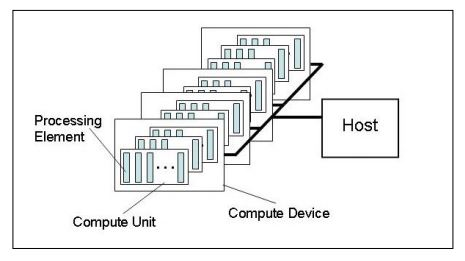
\includegraphics[width=\linewidth]{figures/OpenCL_Platform_Model.JPG}
  \caption{Platform Model in OpenCL}
  \label{fig:opencl1}
\end{figure}
The host device holds the OpenCL application running, from where the commands are submitted to the device, to be executed on the PEs within. The PEs inside a CU execute a single set of instructions as Single Instruction Multiple Data (SIMD) units in parallel. 

\subsection{Memory Model}
Memory directly available to kernels executing on OpenCL devices is known as device memory. The device memory consists of the four distinct memory regions as follows: 
\begin{itemize}
\item \textbf{Global Memory}: This memory region allows read/write access to each work item in all the work groups executing on any device inside a context. Work items are capable of reading from or writing to any part of memory objects. Accesses to global memory may be cached, depending on the device capabilities. \newline\newline
Global memory is shared with all processing elements, and is also available to the host. The host utilises this memory to copy data to/from the device.

\item \textbf{Constant Memory}: This memory region contains content that remains constant throughout the execution of a kernel. \newline\newline
Constant memory is also shared between all processing elements, but it is read-only. It provides an efficient way to share data with all processing elements.

\item \textbf{Local Memory}: A region of memory local to a work group. This region can be used to allot variables that are common to all work items within the work group.\newline\newline
Each CU has its own local memory, only shared with the processing elements within the compute unit. It cannot be accessed by other compute units. 

\item \textbf{Private Memory}: A region of memory private to a work item. Variables declared in one work item’s private memory are not visible to another work item.\newline\newline
Private memory belongs to a single processing element. Each processing element has its own private memory, thereby unable to access all other private memories within or outside the CU.

\begin{figure}[h!]
  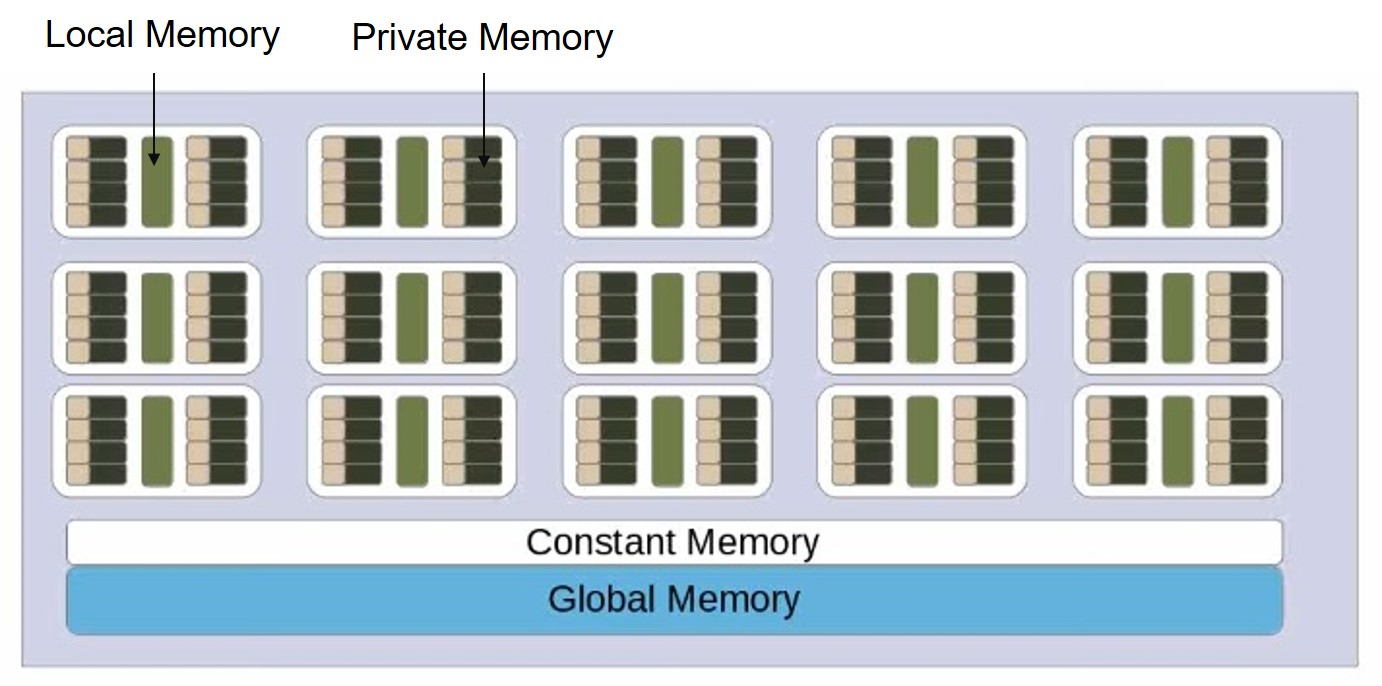
\includegraphics[width=\linewidth]{figures/OpenCL_Memory_Model.jpg}
  \caption{Memory Model in OpenCL \cite{opencl_ajg}}
  \label{fig:opencl2}
\end{figure}
\end{itemize}
Global memory is the only memory which is persistent between kernel calls. Constant, local, and private memories are just scratch spaces, which get reset after every kernel call.

 \subsection{Execution Model}
The core of the OpenCL execution model is based on how kernels execute on the device. The execution of an OpenCL program happens in two parts: kernels that execute on the OpenCL devices, and a host that runs on the host device. The host is responsible for executing kernel functions on the device \cite{opencl_khronos}. These are ordinary functions, albeit with special signatures. The kernel call comprises two parts: an ordinary argument list, and external execution parameters that control the parallelism. OpenCL provides direct support for parallel computing. \newline\newline
\begin{figure}[h!]
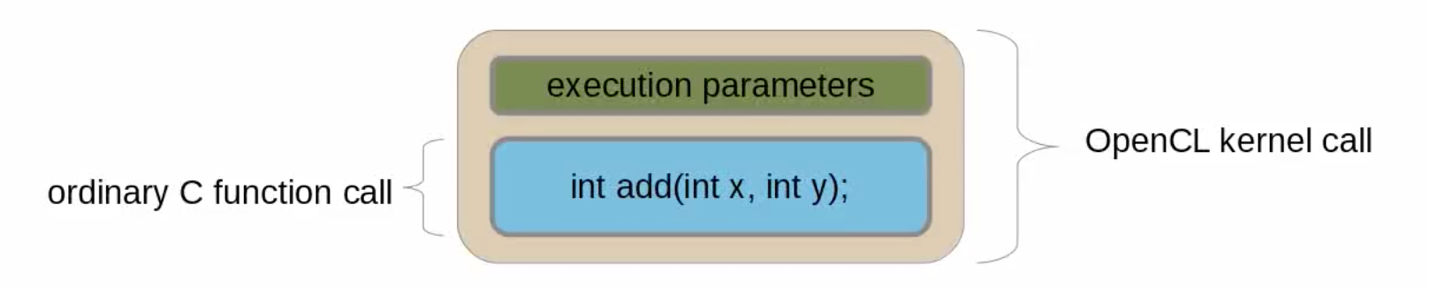
\includegraphics[width=\linewidth]{figures/C_and_OpenCL_Function_Calls.png}
\caption{C and OpenCL Function Calls \cite{opencl_ajg}}
\label{fig:opencl3}
\end{figure}
The host coordinates the execution of the kernels on the OpenCL device. It does not get involved in the computations itself; it only provides execution parameters to launch the kernel and the arguments which the kernel requires for carrying out the operations. 
\subsubsection{Execution Strategy}
The kernel function will be invoked many times, the argument list being identical for all the invocations. This means that the same function gets called repeatedly, based on the execution parameters specified by the host prior to launching the kernel.\newline\newline
There exists an index space provided by an N-dimensional index space. The index space supported in OpenCL is called an NDRange. It can be one, two or three dimensional. Each function invocation can access its index; this is how it is identified. A work item is a kernel invocation for a particular index, and the global id is a unique identity for every work item belonging to the index space. Every work item is provided with a global ID. The global work size is the number of work items in every dimension. The work dimension is the dimension of the index space.\newline\newline 
From the Device Model, the processing elements are the ones which execute the instructions. To be able to execute the kernel multiple times on the device, the work item needs to be mapped to Processing Elements (PEs). Multiple work items are assigned to each PE, so that the case where number of PEs is less than the global work size can be taken care of. \newline\newline
Now, every Compute Unit (CU) has a dedicated local memory which is shared by all PEs within. Local memory provides huge advantages in performance. Thus, work items must be mapped to the PEs in such a way that a group of them can access the local memory of a CU for effective execution. The partitioning of the global work size into smaller pieces leads to the formation of work groups. The work groups provide a more coarse-grained decomposition of the index space. Work groups are assigned a unique work group ID with the same dimension as the index space used for the work items. Work items are assigned a unique local ID within a work group so that a single work item can be uniquely identified by its global ID or by a combination of its local ID and work group ID \cite{opencl_khronos}. \newline\newline
Work groups execute on CUs and share their local memory. All the work items in the work group share local memory and are mapped to PEs within a CU. These work items are capable of identifying which work group they are parts of, work group ID, size of work groups, their global IDs and the global work size. \newline\newline 
The work group size has a device-specific physical meaning. The maximum work group size is a device characteristic. This can be determined by querying the device. Also, it is an integer value; thus, n-dimensional work groups have to be handled in a special way. Work groups are launched by the host device. \newline\newline
The device dependent work group size is a scalar, but work groups can have multiple dimensions. For example, if the maximum work group size is 32, work groups could be launched in 3 dimensions like (8, 2, 2). The following must be true in order to launch the work groups successfully: 
\begin{figure}[h!]
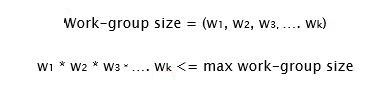
\includegraphics[width=\linewidth]{figures/Work-Group_Size.JPG}
\caption{Handling multi-dimensional work group sizes}
\label{fig:opencl4}
\end{figure} 

The figure below shows an example of how the local size, number of work groups and global size vary for different dimensions of \verb|NDRange|:
\begin{figure}[h!]
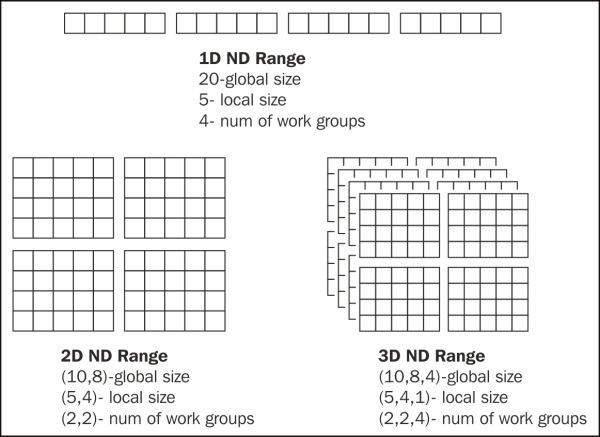
\includegraphics[width=\linewidth]{figures/NDRange_Kernel_Example.jpg}
\caption{NDRange multi-dimensional index space example}
\label{fig:opencl5}
\end{figure}

\subsubsection{Host API}
The host must call certain APIs in order to execute the kernels, which take care of the following:
\begin{itemize}
\item Platform \newline
A platform is an implementation of OpenCL. These are the drivers for specific devices which support the execution of OpenCL kernels. Platforms enables supported devices to be exposed to the programmer. For example, if a system consists of 1 AMD GPU, 1 NVIDIA GPU and an Intel Xeon Phi CPU, all capable of running OpenCL code, there will be three platforms corresponding to each of these devices. The platform is used to discover devices available.
\item Context \newline
A context is created by the host for each platform on which the kernel executes. Thus, a context cannot have multiple platforms. A context acts as a container for devices and memory. Most kernel operations are related to a context.
\item Program \newline
A program is a collection of kernels. A program is loaded by the host device and kernels are extracted from the program to be invoked. The host could either directly compile the OpenCL C code or load a binary representation. Programs are device specific.
\item Asynchronous Device Calls \newline
The host manages devices asynchronously. Host issues commands to the device, telling the device to perform some work. Devices act as slaves and do as the instructed command. The host waits for the commands to complete, meaning that the device has completed the action. Commands can have dependencies on other commands. OpenCL commands are issued by \verb|clEnqueue*| calls. A \verb|cl_event| returned by \verb|clEnqueue*| calls is used for dependencies.

\end{itemize}

 \subsection{Programming Model}
The OpenCL execution model supports data parallel and task parallel programming models. In OpenCL, the primary model is data parallel. \newline

\subsubsection{Data Parallel}
Data parallel programming model (equivalent to SIMD) defines computations in terms of a sequence of instructions applied to multiple elements of a dataset. In a strict data parallel model, a one-to-one mapping exists between a work item and an element in the dataset over which a kernel can be executed in parallel. However, a strict one-to-one mapping is not required in OpenCL. \newline\newline
A hierarchical data programming model exists in OpenCL, where the hierarchical subdivision can be achieved either explicitly or implicitly. In the explicit model, the total number of work items to execute in parallel and how work items are divided among work groups must be defined by the programmer. On the other hand, the implicit model only requires the total number of work items to execute in parallel to be defined, while the division into work groups is taken care by the OpenCL implementation.

\subsubsection{Task Parallel}
Task parallel programming model in OpenCL defines a model in which a single instance of a kernel is executed independent of any index space. It is equivalent to executing a kernel on a compute unit with a work group containing a single work item. It is the simultaneous execution of many different tasks across the same or different memory objects.

\section{Experiments}
A few simple experiments were conducted on different devices – an AMD GPU and an NVIDIA GPU, to see how performance varied on using the same OpenCL kernel code but with different execution parameters. A small kernel which performs 2-dimensional matrix multiplication was written in OpenCL and was launched with different work group sizes on the specific platform to see how its execution varied. \newline\newline
The host device selects the platform and the device, creates the context and command queue, initializes the matrices, creates memory buffers in the device, and transfers the data to the device memory. The two input matrices and one output matrix form the data passed to the kernel function as arguments, on which the matrix multiplication was performed in parallel. The execution is controlled by the \verb|clEnqueueNDRangeKernel| parameters, which define the work group size by specifying the local size and global size. \newline\newline

\begin{equation}
\mathbf{Work\, group\, size = Local\, size}
\end{equation}
The work group size must be perfectly divisible by the specified global work size, failing which the kernel would not be launched and an error would be thrown. \newline\newline
The resultant matrix was stored in a buffer and transferred back to the host asynchronously. The execution time was calculated and the result was compared for correctness by running the matrix multiplication sequentially on the host device. \newline\newline
The following tables show the average timing results on AMD Radeon HD 8730M on platform OpenCL 2.0 AMD-APP (1800.8) and NVIDIA GeForce 405 on OpenCL 1.1 CUDA 4.2.1. \newline
\begin{table}[h!]
\centering
 \caption{Execution time (in µs) of matrix multiplication on AMD Radeon HD 8730M GPU}
 \vspace{3mm}
 \renewcommand\arraystretch{1.3}
 \begin{tabular}{|l|*{5}{r|}}
 \hline
 \multicolumn{6}{|c|}{2-D Matrix Multiplication Timings on AMD GPU} \\
 \hline
 \backslashbox{\bfseries{Local}}{\bfseries{Global}}
 &\makebox[4.5em]{\bfseries{128}}&\makebox[4.5em]{\bfseries{256}}&\makebox[4.5em]{\bfseries{512}}
&\makebox[4.5em]{\bfseries{1024}}&\makebox[5.5em]{\bfseries{2048}}\\
 \hline
 Not Specified & 6121.25 & 48282.5 & 401073.58 & 3270198.86 & 16901530.39\\	
 2 & 8400.23 & 67250.57 & 530250.24 & 1082663.32 & 5365565.08\\
 4 & 2181.05 & 16945.09 & 142875.45 & 298480.89 & 1703353.98\\
 8 & 3359.17 & 25594.24 & 206148.51 & 265741.50 & 1362683.18 \\
 16 & 6123.93 & 48253.26 & 385895.55 & 291104.51 & 1243956.77\\
 32 & Error & Error & Error & Error & Error\\
 64 & Error & Error & Error & Error & Error\\
 128 & Error & Error & Error & Error & Error\\
 \hline
 \end{tabular}
 \label{table:matrix2D_AMD}
\end{table} \newline

\begin{table}[h!]
\centering
 \caption{Execution time (in µs) of matrix multiplication on NVIDIA GeForce 405 GPU}
 \vspace{3mm}
 \renewcommand\arraystretch{1.3}
 \begin{tabular}{|l|*{4}{r|}{c|}}
 \hline
 \multicolumn{6}{|c|}{2-D Matrix Multiplication Timings on NVIDIA GPU} \\
 \hline
 \backslashbox{\bfseries{Local}}{\bfseries{Global}}
 &\makebox[4.5em]{\bfseries{128}}&\makebox[4.5em]{\bfseries{256}}&\makebox[4.5em]{\bfseries{512}}
&\makebox[4.5em]{\bfseries{1024}}&\makebox[5.5em]{\bfseries{2048}}\\
 \hline
 Not Specified & 6138.05 & 48312.10 & 401356.14 & 5773783.80 & Error\\	
 2 & 10721.54 & 58040.95 & 621084.80 & 4527345.84 & Error\\
 4 & 3488.40 & 18654.32 & 232133.67 & 1776133.69 & Error\\
 8 & 2969.30 & 17499.01 & 229669.94 & 1729808.40 & Error \\
 16 & 8382.89 & 34673.16 & 486371.19 & 3369363.59 & Error\\
 32 & Error & Error & Error & Error & Error\\
 64 & Error & Error & Error & Error & Error\\
 128 & Error & Error & Error & Error & Error\\
 \hline
 \end{tabular}
 \label{table:matrix2D_NVIDIA}
\end{table}

Table \ref{table:matrix2D_AMD} and Table \ref{table:matrix2D_NVIDIA} show the execution time (in µs) taken by the two-dimensional matrix multiplication kernel in OpenCL on AMD and NVIDIA GPUs, for different work group sizes (denoted by local size). The global work size was increased from 128 to 2048 and the execution times were measured and noted. \newline\newline
As observed in the results, the AMD Radeon 8730M GPU overpowers the NVIDIA GeForce 405 if their best execution times are compared for different global sizes. Both the devices follow a similar trend for maximum performance (or least execution time). For both the devices, there exists a trend of having a least execution time at a particular work group size, beyond which the increasing the local work size leads to higher execution times (lower performance). In the case of AMD Radeon 8730M, the best performance is achieved when the work group size is 4, while for NVIDIA GeForce 405 it is 8. These best performing work group size values are device specific, as seen from the results. \newline\newline
Upon further increasing the work group size, it was noticed that the execution of OpenCL kernel was failing due to error in launching it. This work group size was 32 for both AMD Radeon 8730M and NVIDIA GeForce 405. This falls in line with the Section 4.1.3.1 Execution Strategy, which mentions that the maximum work group size is device-specific. Thus, we can conclude that the maximum work group size for both the GPUs is 16. \newline

\chapter{Convolutional Neural Networks}
\label{ch5_cnn}

Convolutional Neutral Network (CNN) is a classification of multi-layered neural networks \cite{cnn_lecun_lenet5}. CNNs have excellent performance in areas such as image recognition and classification.  CNNs are at the core of state-of-the-art approaches to a variety of computer vision tasks, including image classification \cite{kriz_suts_hinton_nips2012} and object detection \cite{gir_don_dar_mal_cvpr2014}. They are widely used in the detection and identification of faces, objects and animals, apart from powering robot vision and driverless cars \cite{cnn_karn}. LeNet-5 is one such model designed for handwritten and machine-printed character and digit recognition.

\section{Introduction}
\label{sect5_1}

\subsection{Neural Networks}
\label{sect5_1_1}
An Artificial Neural Network, simply put as Neural Network, is a computational model motivated by the manner in which neural networks in the human brain and nervous system process information \cite{cnn_karn}. The field of Neural Networks was primarily inspired by the objective of modeling biological neural systems, but has since diverged and become a part of engineering and achieving great results in machine learning \cite{nn_stanford_1}. \newline\newline The fundamental building block of a neural network is the neuron, also referred to as node. The following figures shows a biological neuron and its computational model are related: \newline

\begin{figure}[h!]
\centering
\includegraphics[width=8cm]{figures/Neuron.png}
\caption{Representation of a biological neuron\cite{nn_stanford_1}}
\label{fig:cnn1}
\end{figure}

\begin{figure}[h!]
\centering
\includegraphics[width=7cm]{figures/Neuron_Model.jpg}
\caption{Computational model of a neuron \cite{nn_stanford_1}}
\label{fig:cnn2}
\end{figure}

In this model, a node gets inputs from other node or an external source, and calculates an output. Inputs have associated weights assigned on basis of their relevance to other input nodes. The node applies a function on the weighted sum of inputs, as shown in Figure \ref{fig:cnn3}.
\begin{figure}[h!]
\centering
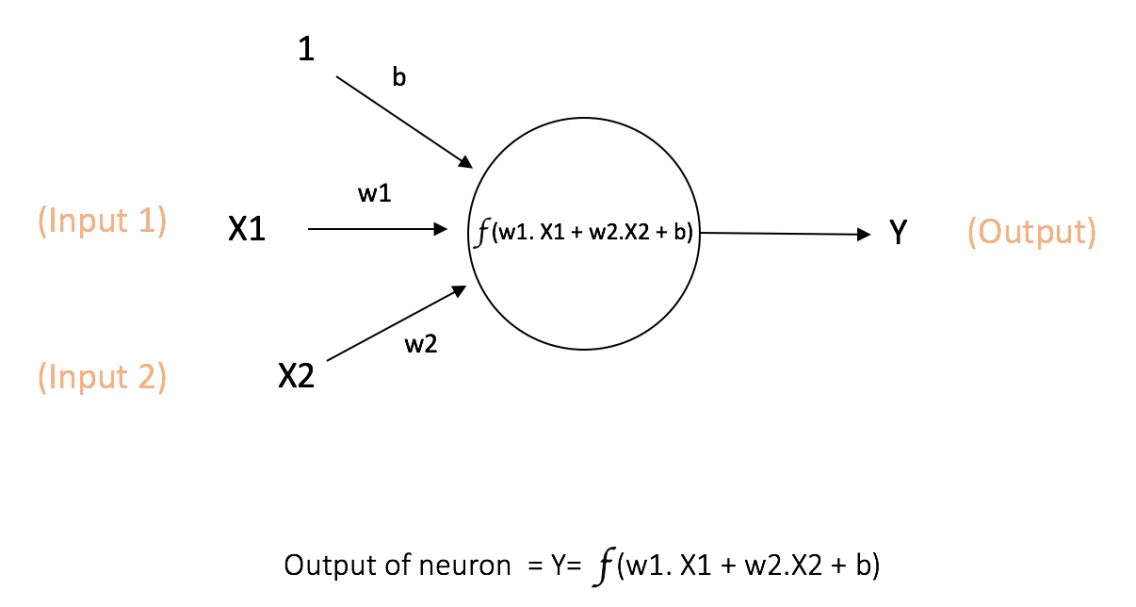
\includegraphics[width=10cm]{figures/Input_and_Output_to_a_Node.png}
\caption{Computation in a Neuron\cite{nn_karn}}
\label{fig:cnn3}
\end{figure}

The neuron receives inputs x1 and x2 with weights w1 and w2. Each neuron also has another input 1, with a weight \textbf{bias} associated with it. The bias value provides each node a trainable constant value.\newline\newline 
The function applied to the sum of weighted inputs, known as Activation Function, is a non-linear function introduced to force neurons to learn non-linear representations, as most of real world data is non-linear. Following are some common activation functions used:

\begin{itemize}
\item Sigmoid \newline
Takes a real-valued input and squeezes it in the range 0 to 1
\begin{equation}
\mathbf{\sigma(x) = 1 / (1 + exp(-x))}
\end{equation}

\item tanh \newline
Takes a real-valued input and squeezes it in the range -1 to 1
\begin{equation}
\mathbf{tanh(x) = 2 \sigma (2x)-1}
\end{equation}

\item ReLU \newline
Takes a real-valued input and thresholds it at zero (replaces negative values with zero)
f(x) = max(0, x)
\begin{equation}
\mathbf{f(x) = max(0, x)}
\end{equation}
\end{itemize}

\subsubsection{Feedforward Neural Network}
\label{sect5_1_1_1}
One of the first and simplest neural networks devised was the feedforward neural network. There are multiple neurons placed in layers, with edges connecting them. Each of these edges are tagged a weight. Figure \ref{fig:cnn4} shows an example of a feedforward neural network.\newline\newline
\begin{figure}[h!]
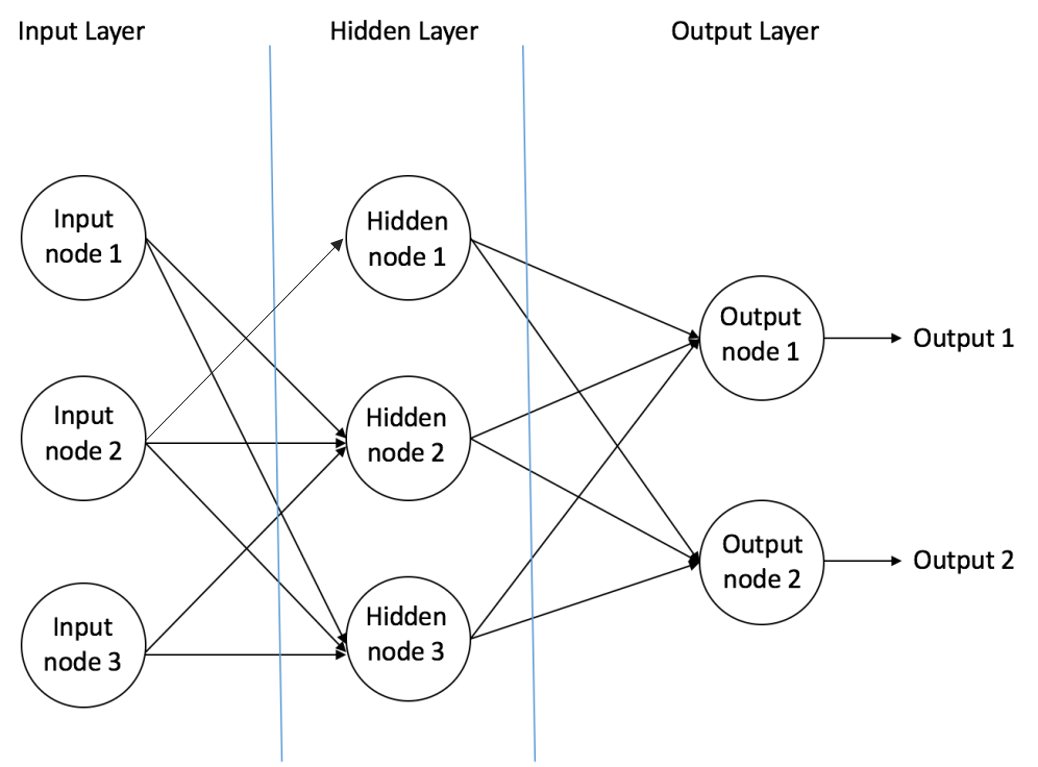
\includegraphics[width=14cm]{figures/Feedforward_Neural_Network.png}
\caption{Feedforward Neural Network \cite{nn_karn}}
\label{fig:cnn4}
\end{figure}
Information only moves in the forward direction in a feedforward neural network. Input nodes receive signals from the outside world and pass on the information forward to the hidden nodes, which perform computations and propagate information to the output nodes. The output nodes carry out some calculations and transfer the result to the outside world. There can only be one input and output layer of nodes, but multiple hidden layers of nodes in a feedforward neural network.\newline\newline 
They are of two types, \textbf{Single Layer Perceptron} and \textbf{Multi Layer Perceptron} (MLP). The former does not consist of any hidden nodes in the middle, while the the latter has at least one hidden layer. MLPs are very useful in several practical learning applications.
\subsubsection{Training}
\label{sect5_1_1_2}
For any neural network to accurately learn relationships between inputs and outputs and generate correct predictions, training is required. For an MLP to learn, back propagation algorithm is used.\newline\newline
Back-propagation is one of the many ways to train a MLP. It is a supervised learning algorithm which learns from labeled training datasets. Back-propagation algorithm trains the MLP by correcting its output when a mistake is made. Its objective is to assign correct weights to the connections between nodes in different layers, so as to generate accurate outputs. \newline\newline
In the beginning, all edge weights are assigned random values. For every input in the training dataset, the MLP is activated and its output is noticed and checked against the desired output from the labeled data. The error is then “propagated” back to the previous layer. This error is computed and the weights are updated. This process repeats until the output error is less than a pre-specified threshold.\newline\newline
Once the algorithm finishes, a “learned” neural network is created which can work with new inputs. It will have learned from millions of example inputs (labeled data) and from mistakes made in predicting outputs (error propagation).


\subsubsection{Visualisation}
\label{sect5_1_1_3}
Andy Harley developed a two-dimensional and three-dimensional representation of an MLP trained to recognise the handwritten digits from the \ac{MNIST} database \cite{harley2015isvc}. The following figure shows how a MLP is visualised in 3D.

\begin{figure}[h!]
\centering
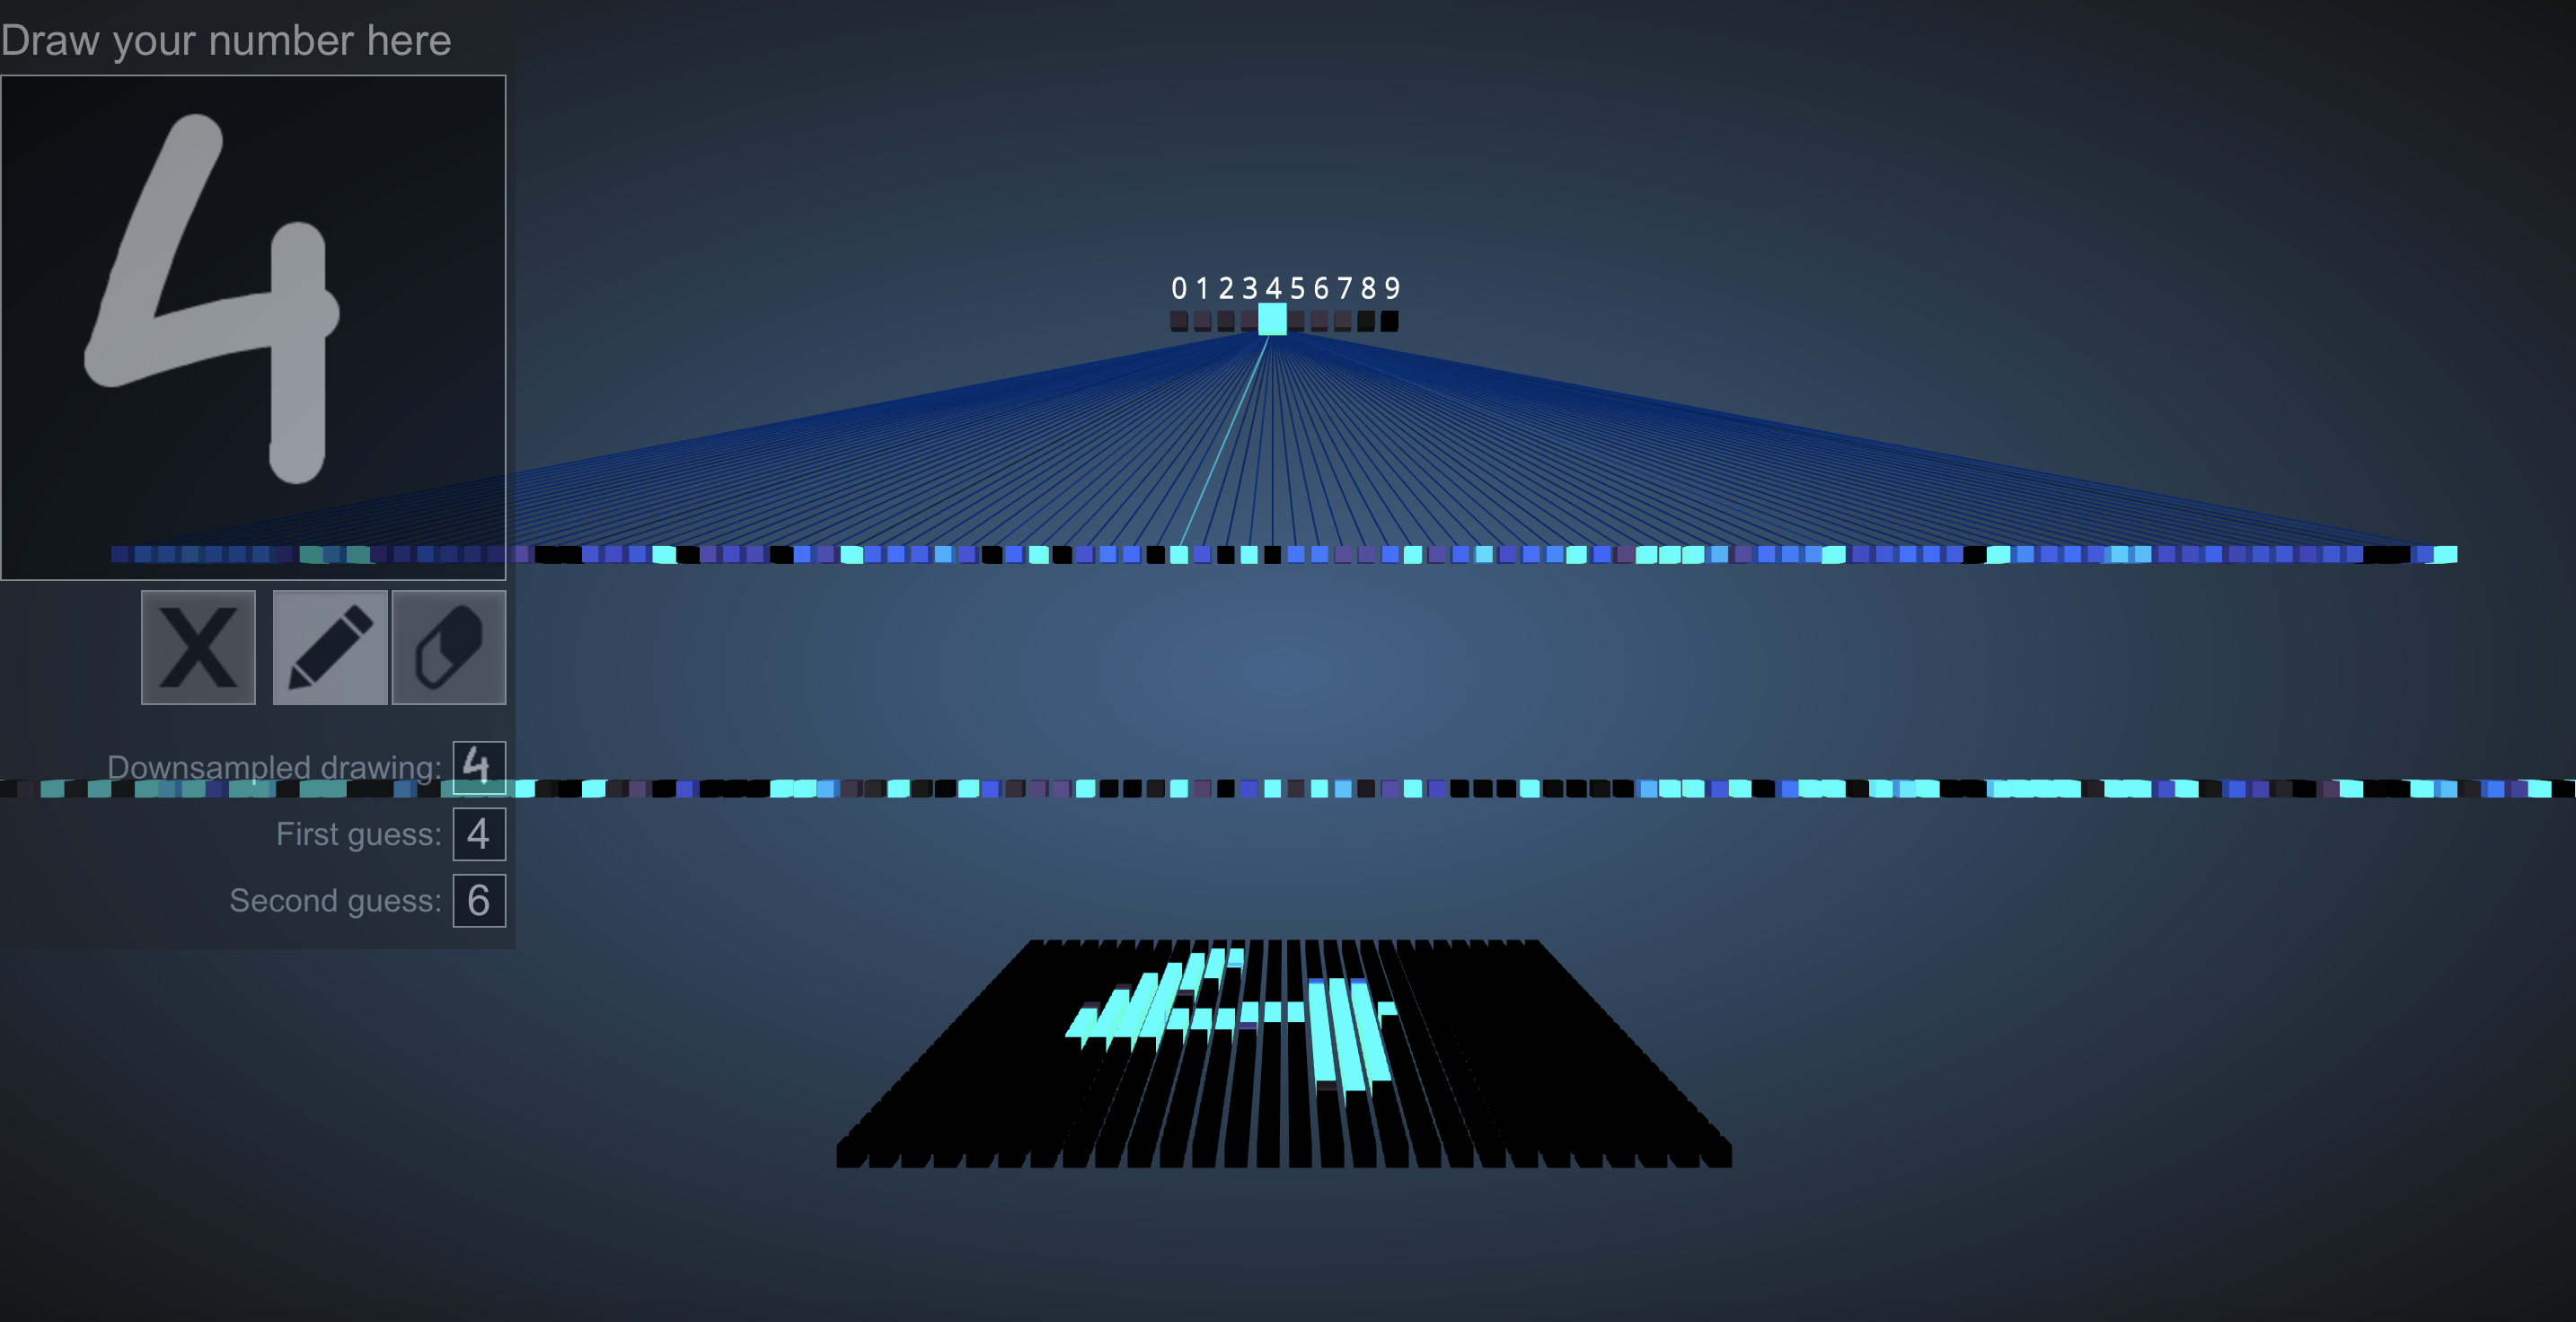
\includegraphics[width=12cm]{figures/Fully_Connected_MLP_3D.png}
\caption{3D Visualisation of a fully connected MLP \cite{harley2015isvc}}
\label{fig:cnn5}
\end{figure}

This MLP network has 784 nodes on the bottom layer (corresponding to pixels), 300 nodes in the first hidden layer, 100 nodes in the second hidden layer, and 10 nodes in the output layer (corresponding to the 10 digits)\cite{harley2015isvc}. \newline\newline
A brighter colour corresponds to a node which has a higher output value than others. In the input layer, the bright nodes are the ones receiving higher numerical pixel values as input. In the output layer, the only bright node corresponds to the digit 4, indicating that the MLP has correctly classified the input digit as 4.

\subsection{Convolutional Neural Networks}
\label{sect5_1_2}
CNNs are quite similar to regular neural networks – they are composed of neurons possessing learnable weights and biases; neurons get inputs, perform dot products and follow it up with non-linearity (optionally). The network expresses a single differentiable score function: from the raw image pixels on one end to class scores at the other. There is a loss function on the last, fully-connected layer which generates the final output. The difference exists for the type of input CNN architectures explicitly assume, which are images, allowing certain properties to be encoded into the architecture. These then make the forward function more efficient to implement and hugely decrease the number of parameters in the network \cite{cnn_stanford}.

\subsubsection{Architecture}
\label{sect5_1_2_1}
CNNs are biologically-inspired variants of MLPs. They take benefit of the fact that inputs accepted are images, and constrain the architecture in a more sensible way. Unlike a regular Neural Network, the layers of a CNN consist of neurons arranged in 3 dimensions: width, height, depth. Neurons in a layer are only be connected to a small region of the layer before it, instead of all neurons in a fully-connected way.Every layer transforms a 3D input to 3D output using some differentiable function. Eventually, the final output layer is one-dimensional, as the full image gets reduced into a single vector of class scores by the end of all processing.

\begin{figure}[h!]
\centering
\includegraphics[width=6cm]{figures/Neural_Net.png}
\hspace{7mm}
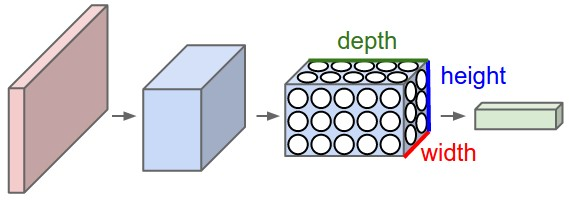
\includegraphics[width=6cm]{figures/cnn.png}
\caption{Visualisation of a Feedforward neural network \textit{(left)} and a CNN \textit{(right)}}
\label{fig:cnn6}
\end{figure}

For accuracy in predictions made by neural networks, a lot depends on how the layers are defined by the architecture. In our case, we are going to study the LeNet-5 architecture. 

\subsection*{LeNet-5 Architecture}
\label{sect5_1_2_1a}

This was one of the very first convolutional neural network, conceptualised in 1994, which propelled the field of Deep Learning. Yann LeCun, a French scientist was the person behind this pioneering work, achieved as a result of several successful iterations since 1988 \cite{cnn_culurciello}. Several new architectures have been proposed in the recent years which have improved features over LeNet, but they are all based upon the foundation of Lenet. \newline\newline
The network receives an image as an input and assigns probabilities to various output possibilities. The one with the highest probability is the classified character or digit. Following are the various steps involved in the classification process:
\begin{figure}[h!]
\centering
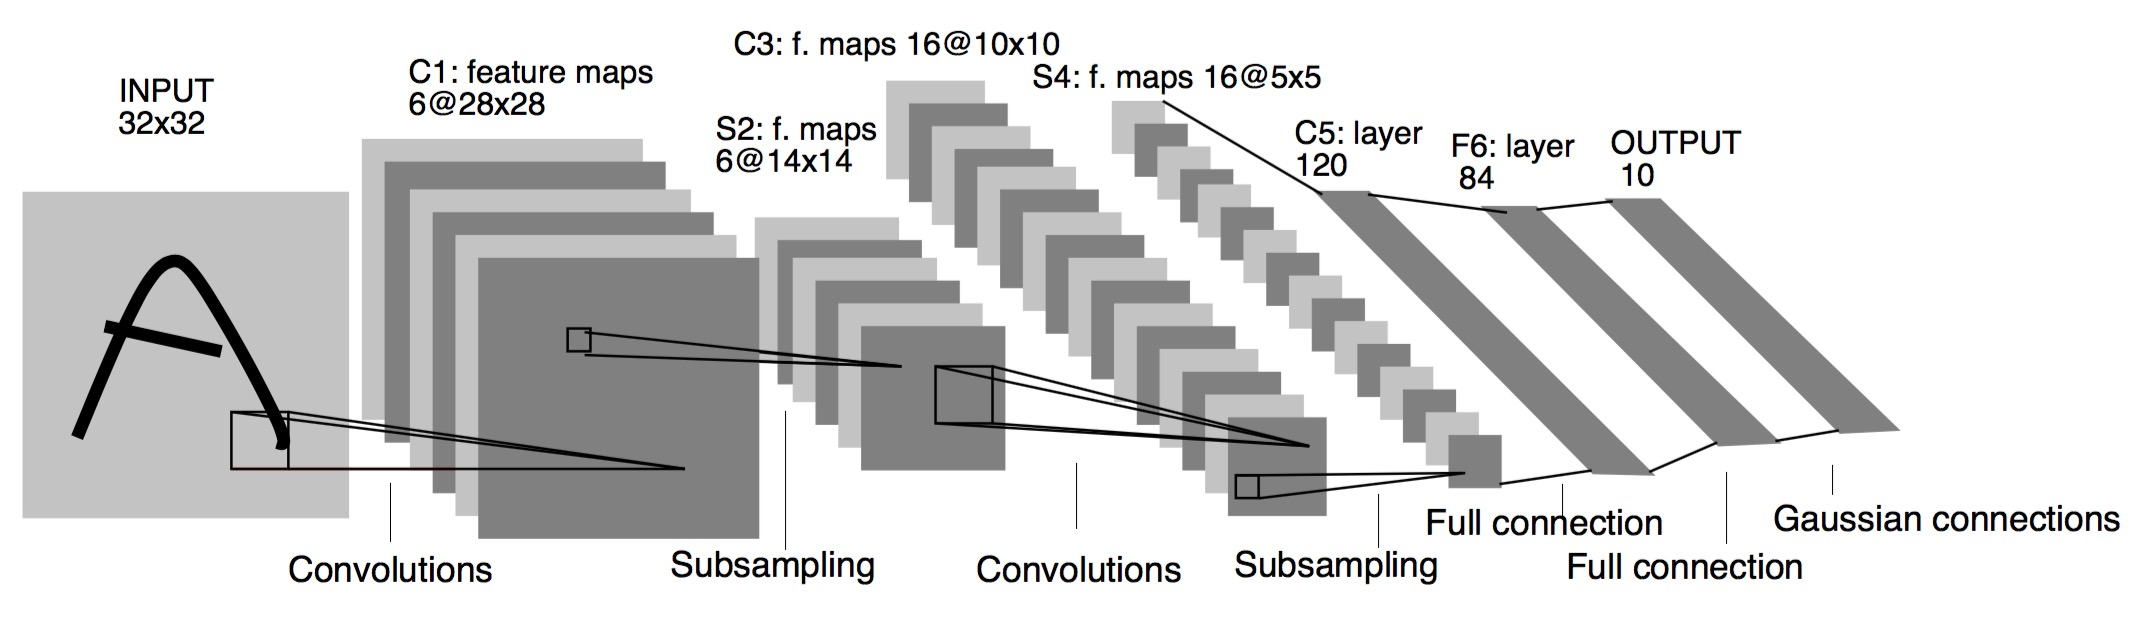
\includegraphics[width=\linewidth]{figures/Lenet5.png}
\caption{Lenet-5 architecture}
\label{fig:cnn7}
\end{figure}

The operations forming the building blocks of every convolutional neural network are as follows:
\begin{itemize}
\item Convolution
\item Pooling or Down-Sampling
\item Activation Function for Non Linearity (ReLu)
\item Classification (Fully Connected Layer)
\end{itemize}

\subsubsection*{Convolution Layer}
\label{sect5_1_2_1a_a}
Channel is a traditional term used to refer to a the coloured component of an image. A coloured image from a has three channels – red, green and blue, and could be imagined as three 2D-matrices stacked over each other (one for each color), each having pixel values in the range 0 to 255.\newline\newline
On the other hand, grayscale images have just one channel. The value of each pixel in the matrix will range from 0 to 255 – zero indicating black and 255 indicating white. Convolution layer extracts key features from the input image using convolution operations. It preserves the spatial relationship between pixels by learning image features using small squares of input data.\newline\newline
The image is convolved with multiple filters, resulting in the formation of different feature maps. Essentially, each filer is a 2D matrix (for a grayscale image), based on the value of whose individual elements, feature maps vary. \newline\newline
The orange matrix is slided over the image matrix, 1 pixel  at a time (also called ‘stride’), and for each position, an element wise multiplication is computed (between the two matrices). The multiplication outputs are added to get the final integer which makes one element of the output matrix at the corresponding position. The 3×3 filter only observes one part of the input image in each stride.\newline\newline
For example, if there is a 5x5 image convolved with a 3x3 filter as follows, a feature map will be generated based on the convolution result. For a different filter matrix, another feature map would have been generated.\newline\newline
\begin{figure}[h!]
\centering
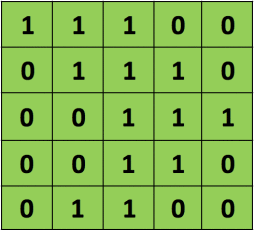
\includegraphics[width=3cm]{figures/Image.png}
\hspace{4mm}
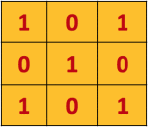
\includegraphics[width=3cm]{figures/Filter.png}
\caption{Convolution operation in action - a 5x5 Image  and a 3x3 filter}
\label{fig:cnn8}
\end{figure}

\begin{figure}[h!]
\centering
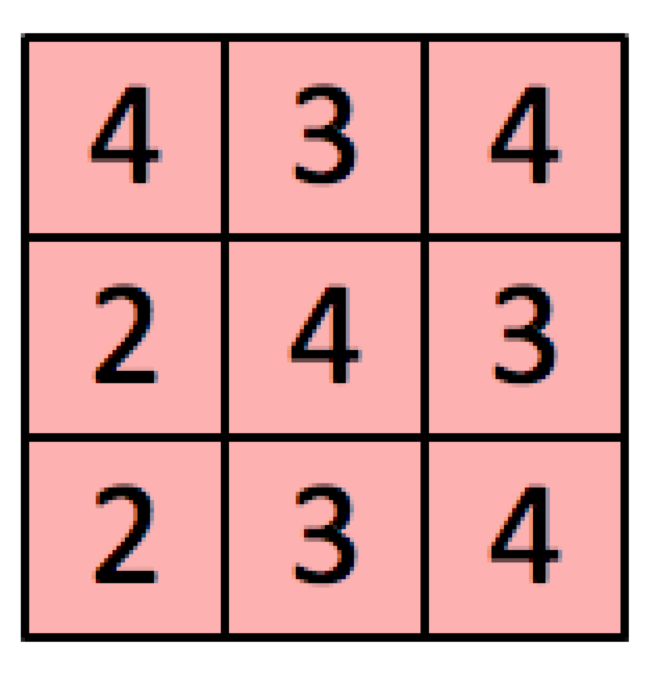
\includegraphics[width=3cm]{figures/Convolution_Result.png}
\caption{Convolution operation in action - a 5x5 Image  and a 3x3 filter}
\label{fig:cnn9}
\end{figure}

In the practical world, a CNN learns the values or weights of these filters itself during the training process. The greater the number of filters, the more image features are extracted and the better the network becomes at recognizing patterns in images, not seen previously.


\subsubsection*{Pooling Layer}
\label{sect5_1_2_1a_b}
Pooling or down-sampling reduces the dimensions of each feature map but retains the most important details. It could be done using different mathematical operations: addition, average or maximum.\newline\newline
In case of Max Pooling, a spatial neighborhood is defined (for example, a 2×2 window) and the largest element is taken from the rectified feature map within that window.
\begin{figure}[h!]
\centering
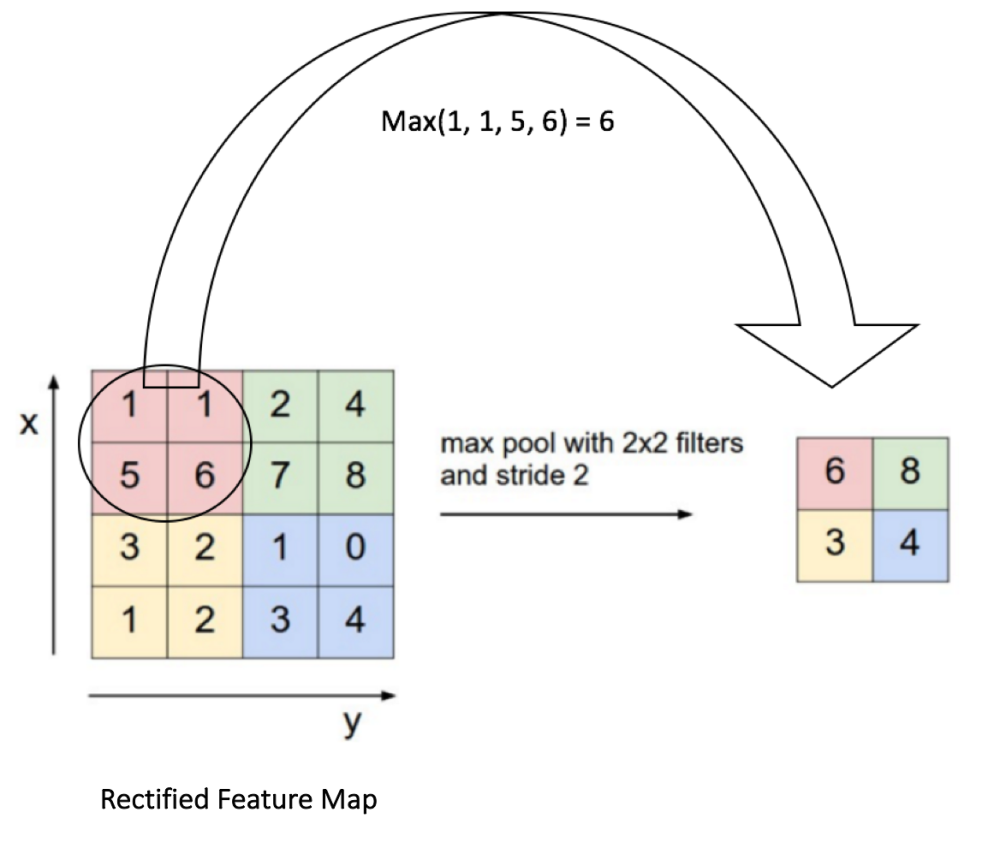
\includegraphics[width=8cm]{figures/Max_Pooling.png}
\caption{Demonstration of Max Pooling}
\label{fig:cnn10}
\end{figure}
The dimensionality of the 2-dimensional window (2x2) is also called as stride. The window is slided by the stride value, and the maximum value from that region is taken in the reduced feature map. This is how the dimensionality of the feature map decreases. Figure \ref{fig:cnn9} demonstrates how pooling reduces the size of the feature map for a sample image.
\begin{figure}[h!]
\centering
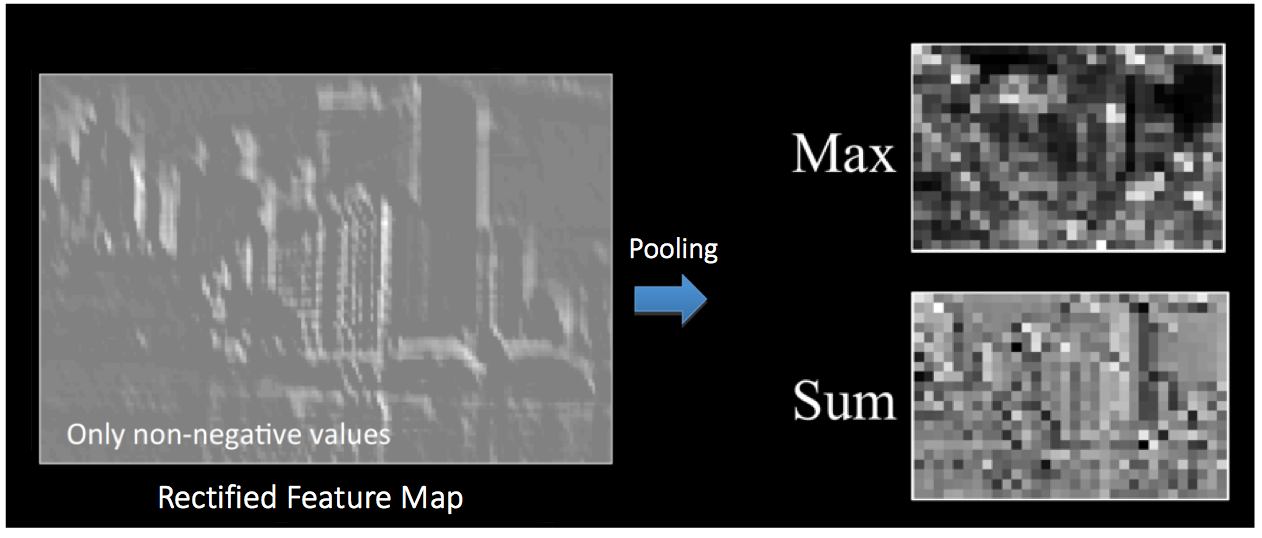
\includegraphics[width=10cm]{figures/Effect_Pooling.png}
\caption{Effect of Max Pooling layer on a sample image}
\label{fig:cnn11}
\end{figure}

\subsubsection*{Non-Linearity Layer (ReLU)}
\label{sect5_1_2_1a_c}
This is an additional layer utilised to introduce non-linearity in the image feature maps. ReLU stands for Rectified Linear Unit, which is a non-linear function.
\begin{equation}
\mathbf{Output = max(0, input)}
\end{equation}
\begin{figure}[h!]
\centering
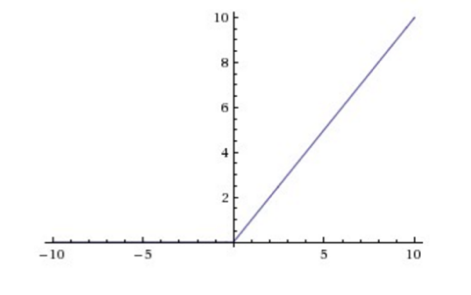
\includegraphics[width=8cm]{figures/ReLu_Layer.png}
\caption{Non-linearity operation in ReLU layer}
\label{fig:cnn12}
\end{figure}\newline
This operation is done on every single element of the image or its feature map(s), replacing every negative value with a zero.
\begin{figure}[h!]
\centering
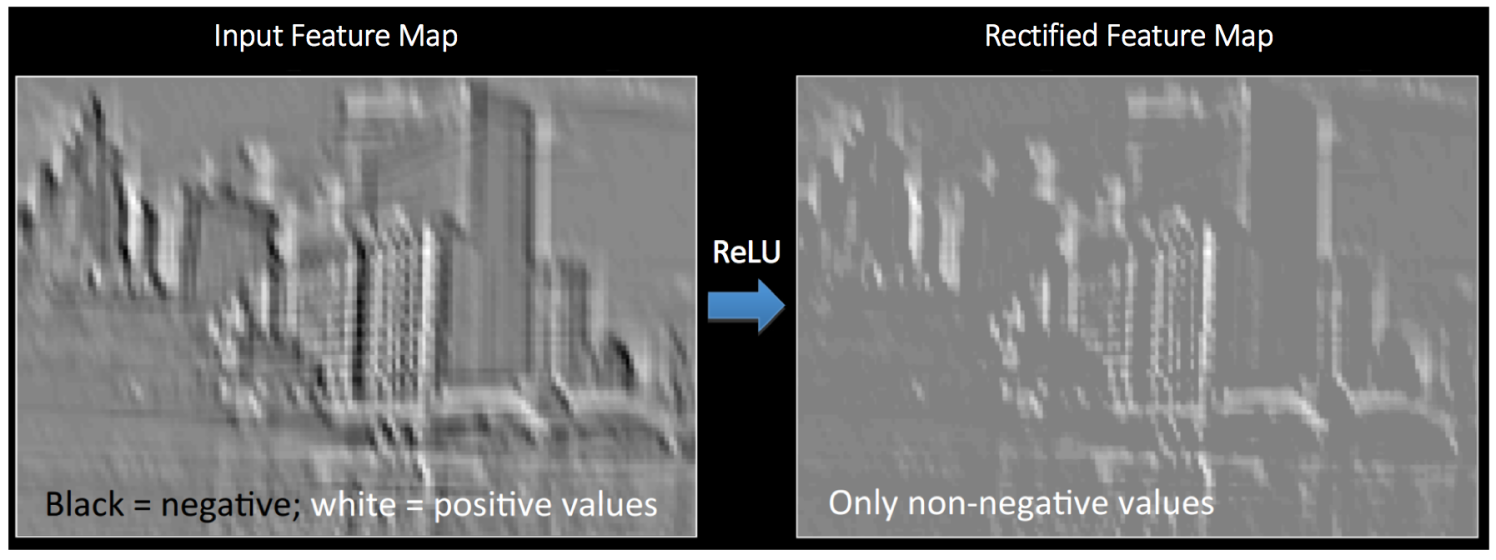
\includegraphics[width=12cm]{figures/Effect_ReLu.png}
\caption{Effect of ReLU layer on a sample image}
\label{fig:cnn13}
\end{figure}
The purpose of ReLU is to introduce non-linearity in our CNN, since most of the real-world data the network would be classifying would be non-linear. Other non-linear functions such as \textbf{tanh} or \textbf{sigmoid} could also be used as an alternative. Figure \ref{fig:cnn11} shows the effect of applying non-linearity on an image.

\subsubsection*{Fully Connected Layer}
\label{sect5_1_2_1a_d}

The fully connected layer is a classic \ac{MLP} using a softmax activation function in the output layer. Each node from the previous layer is connected to each node in the the next layer, hence the term "fully connected".\newline\newline
The output from the convolutional and pooling layers represent high-level features of the input image. The purpose of this fully connected layer is to use these features for classifying the input image into various categories, depending on the training data. \newline\newline
The sum of output probabilities from the Fully Connected Layer is 1. This is ensured by using the \textbf{softmax} as the activation function in the output layer of the Fully Connected Layer. The \textbf{softmax} function takes a vector of arbitrary real-valued scores and squashes it to a vector of values between zero and one that sum to one.

\subsection*{Training}
\label{sect5_1_2_1b}
The training of a CNN follows the same methods as those for a regular neural network. All filters and weights are assigned with random values. The network then accepts an image as its input and performs the convolution, pooling, and non-linearity operations, calculating its output probability in the end. This prediction may or may not be accurate, since the weights were assigned randomly.\newline\newline
The total error is computed at the output layer. Afterwards, back propagation is used to calculate the gradients of the error with respect to all weights in the network and gradient descent is used to update the values of all weights to minimise the output error. The weights are updated in proportion to their contribution to the total error. \newline\newline
These steps are repeated across all images present in the dataset to train the CNN completely, which results in a "learned" network. 
\subsubsection{Visualisation}
\label{sect5_1_2_2}
Along with visualising \ac{MLP}, Andy Harley developed a visualisation tool for a CNN trained to recognise handwritten digits from the MNIST database \cite{harley2015isvc} as well. \newline\newline
The following figure shows how a network can be visualised in 2D.

\begin{figure}[h!]
\centering
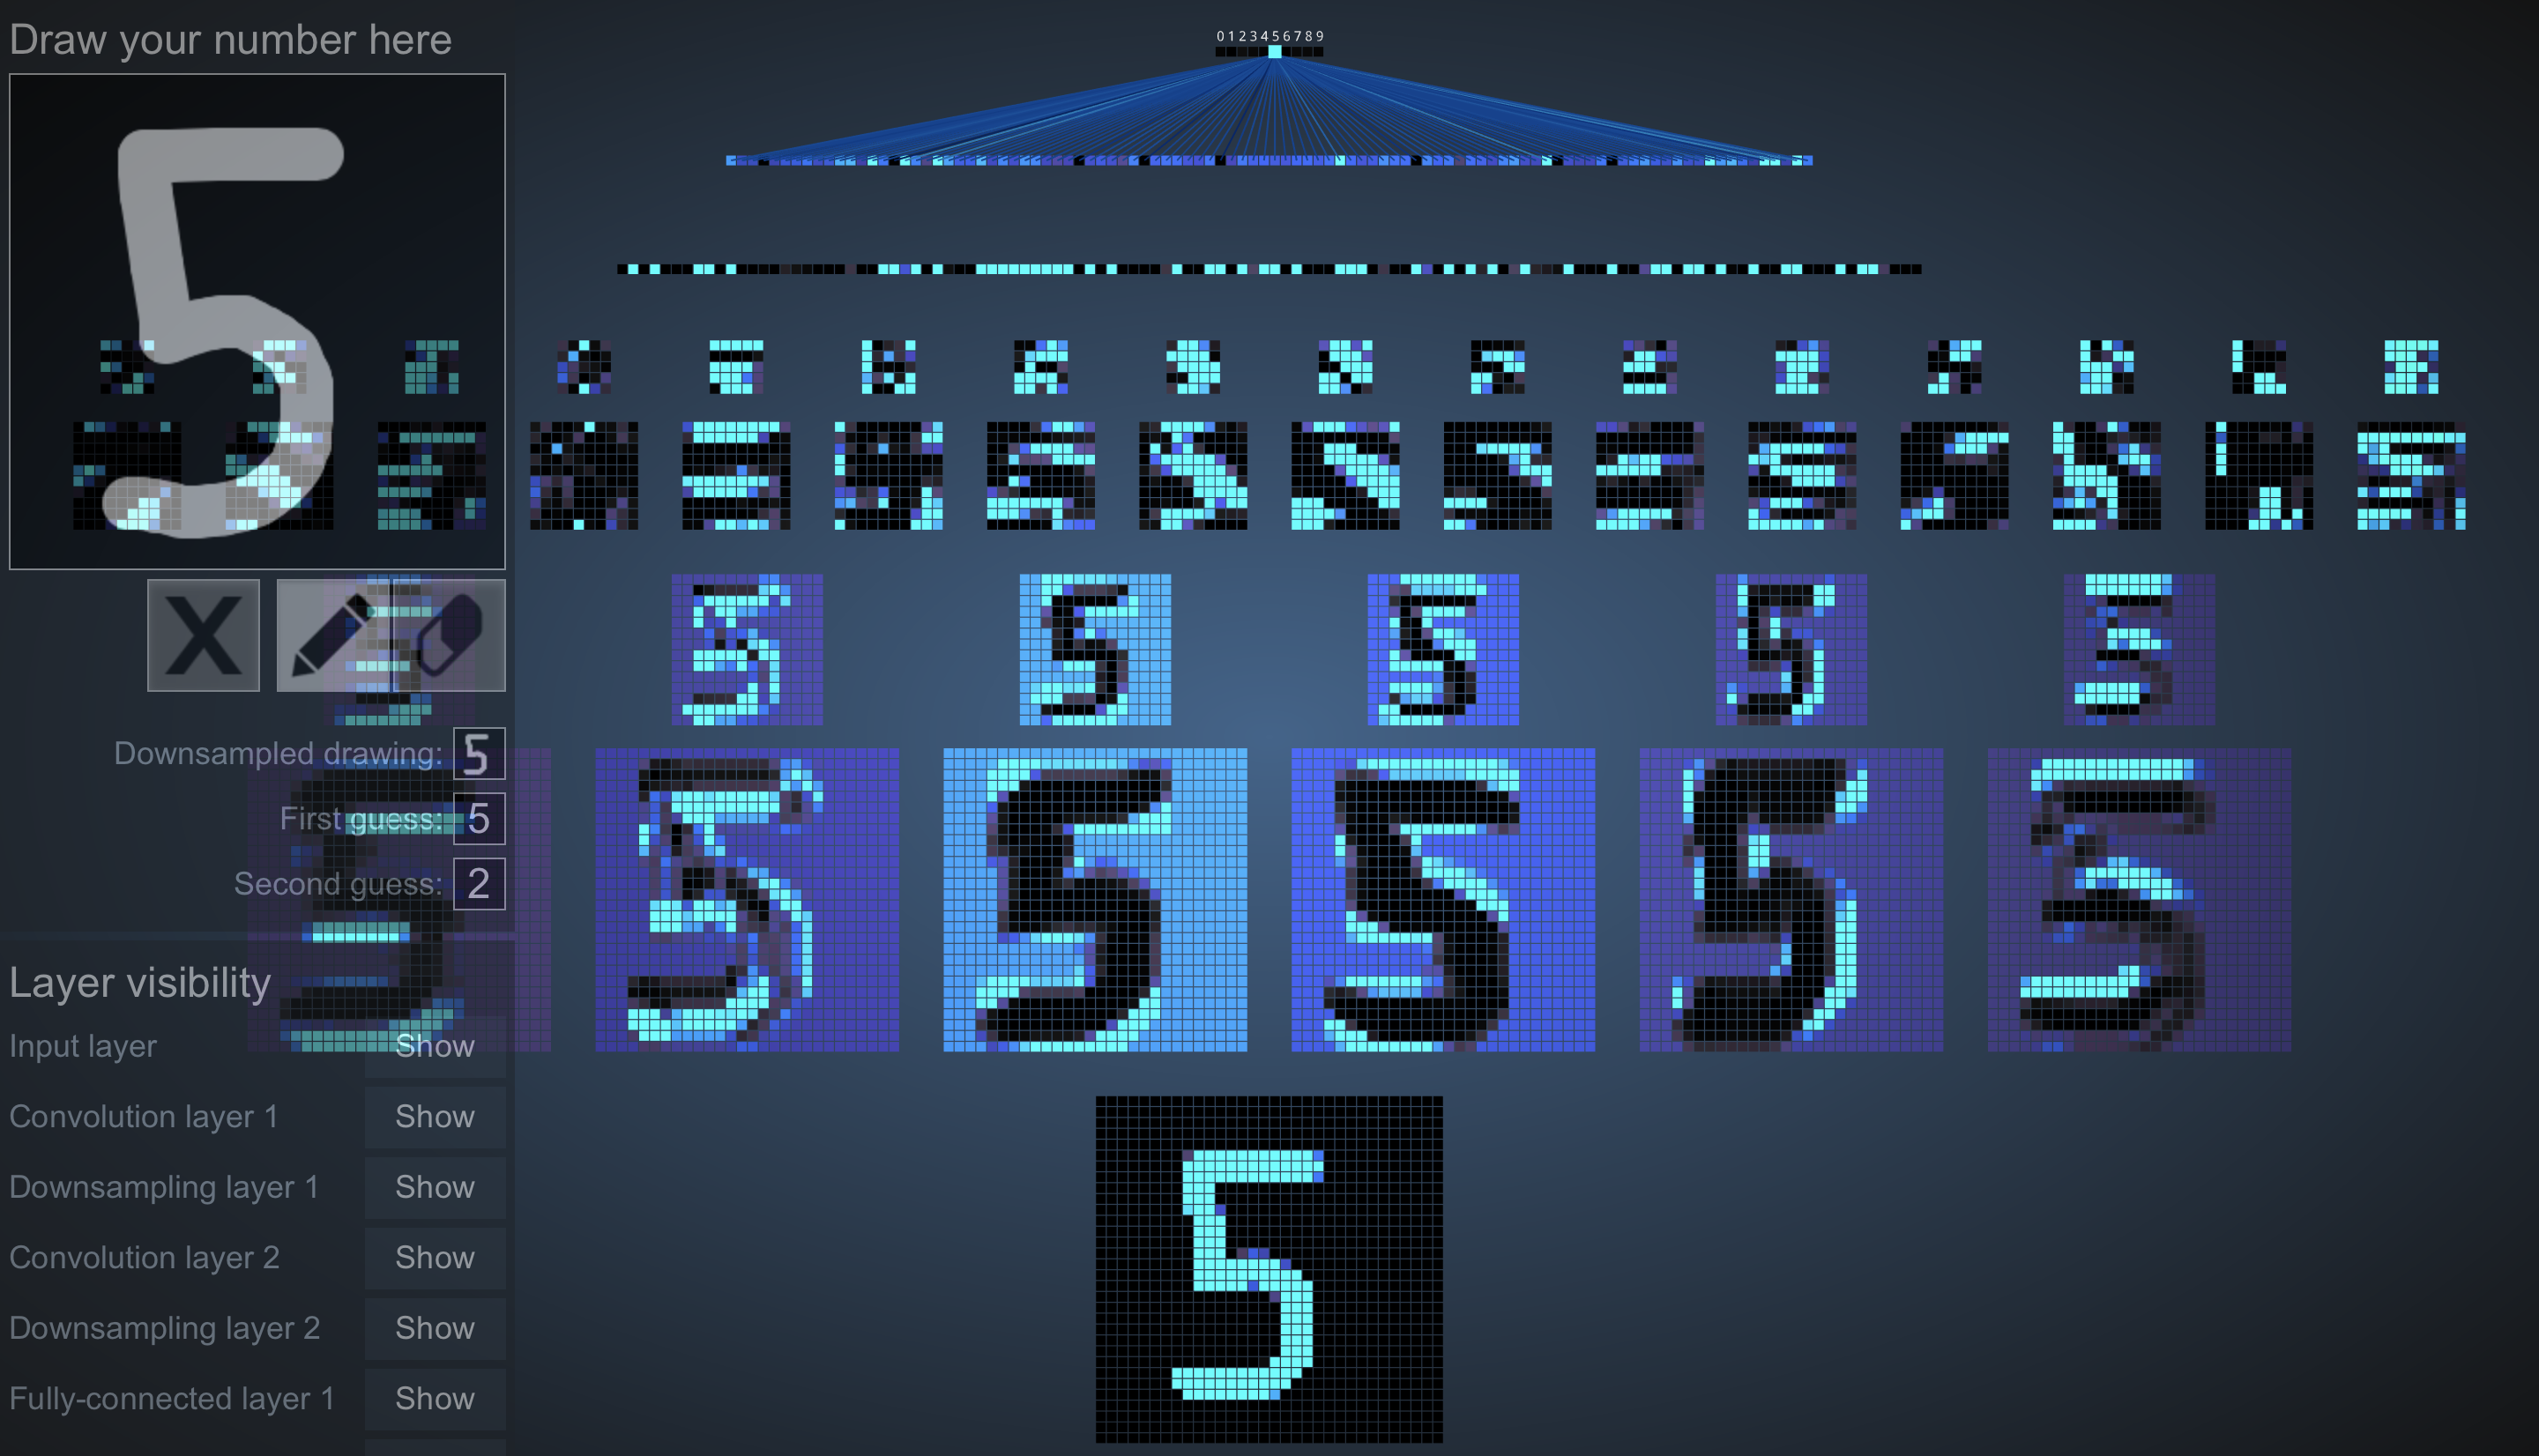
\includegraphics[width=13cm]{figures/ConvNet_2D.png}
\caption{2D Visualisation of a CNN recognising MNIST handwritten digits \cite{harley2015isvc}}
\label{fig:cnn14}
\end{figure}

This CNN has 1024 nodes on the bottom layer (corresponding to pixels), six 5x5 (stride 1) convolutional filters in the first hidden layer, followed by sixteen 5x5 (stride 1) convolutional filters in the second hidden layer, then three fully-connected layers, with 120 nodes in the first, 100 nodes in the second, and 10 nodes in the third. The convolutional layers are each followed by a downsampling layer that does 2x2 max pooling (with stride 2)\cite{harley2015isvc}.

\section{MNIST Database}
\label{sect5_2}
The \ac{MNIST} database is an enormous database of handwritten digits which is frequently utilized for training different image processing procedures \cite{mnist_wiki}. It is also extensively used for training and testing in the field of machine learning. \newline\newline 
The MNIST database consists of 60,000 training and testing images \cite{mnist_kus_ernst}. Samples from National Institute of Standards and Technology’s (NIST) original training and testing dataset were remixed to generate the MNIST database. The digits have been size-normalized and centered in a fixed-size image of 20x20 while preserving their aspect ratio \cite{cnn_lecun_mnist_app}. The resulting images contain grey levels because of anti-aliasing methods used by the normalization algorithm. The images were centred in a 28x28 image by calculating the centre of mass of the pixels and rendering the image to place this point at the centre of the 28x28 field. \newline\newline
The database is a good starting point for individuals who desire to learn machine learning techniques and pattern recognition methods on real-world data while spending marginal efforts on preprocessing and formatting. When one learns how to program, there's a tradition to print "Hello World" in his first program. Similar to how programming has Hello World, machine learning has MNIST. \newline\newline
A number of scientific papers have been written to attempt achieving the lowest error rate in predicting the digits – one paper achieves a rate as low as 0.23 percent using a hierarchical system of convolutional neural networks.

\section{Experiments}
\label{sect5_3}
An existing real word application was obtained and executed to further gauge the performance capabilities of OpenCL. An MNIST handwritten digits prediction application written by Gopala Krishna Hegde based on LeNet-5 convolutional neural networks was cloned from GitHub for this purpose \cite{cnn_mnist_papaa}. The implementation has been done in C++ as well as OpenCL.

\subsection{Analysis of Application Code}
\label{sect5_3_1}
After understanding how the LeNet-5 architecture works, the application was studied and the sizes and computations of the various layers within the CNN were determined. For each layer, mathematical operations like add, substract, multiply, divide and finding the maximum of two numbers were counted as operations.\newline\newline
The layers in the network can be represented as follows:
\begin{figure}[h!]
\centering
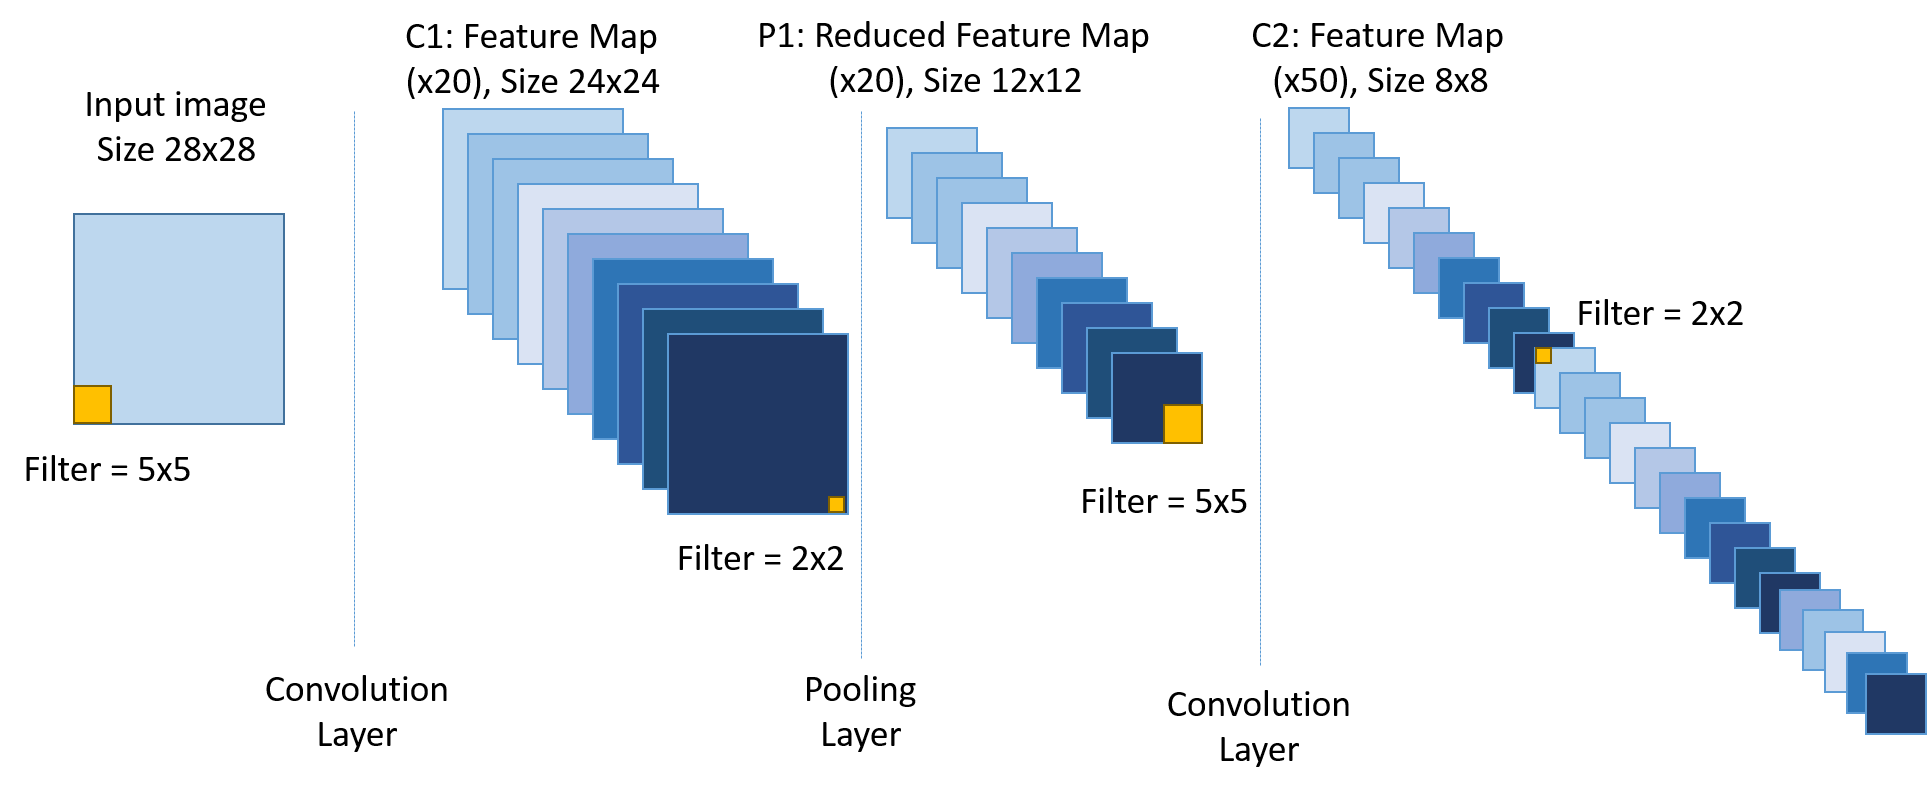
\includegraphics[width=13cm]{figures/Papaa_LeNet5-1.png}
\caption{Representation of the classification process - \textit{Part 1}}
\label{fig:cnn14}
\end{figure}

\begin{figure}[h!]
\centering
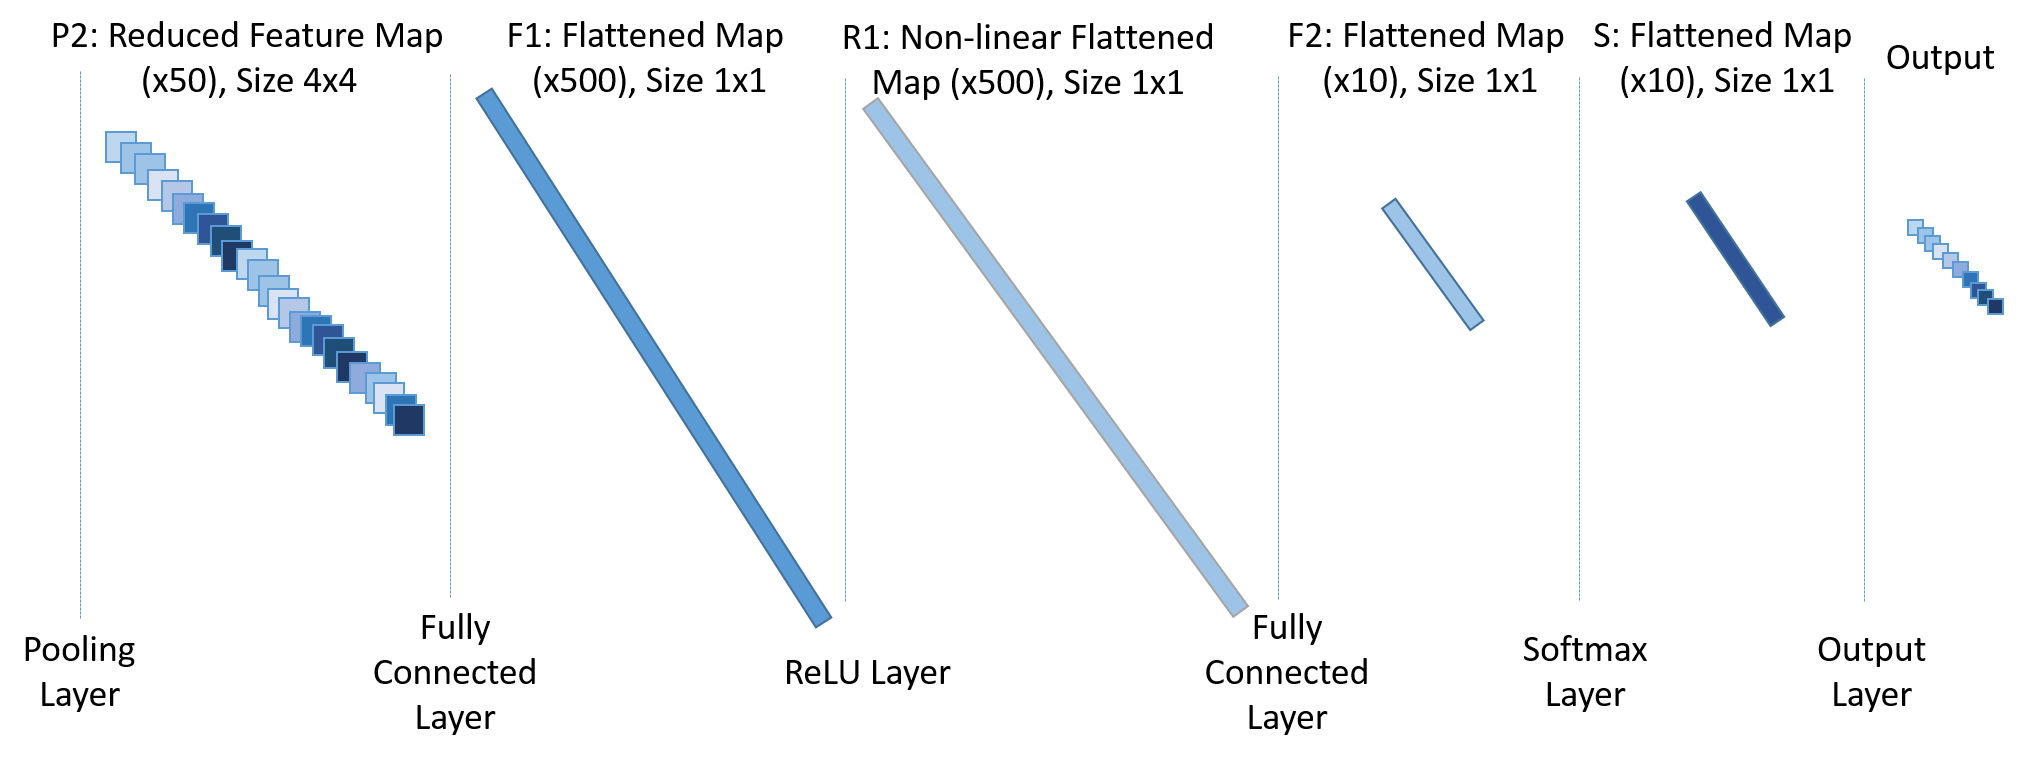
\includegraphics[width=\linewidth]{figures/Papaa_LeNet5-2.png}
\caption{Representation of the classification process - \textit{Part 2}}
\label{fig:cnn16}
\end{figure}

The following table indicates the use of various layers from the LeNet-5 architecture in this application. Each layer has an input size, output size and number of computations associated with it.\newline

\begin{table}[h!]
\centering
 \caption{Characterisitics of LeNet-5 layers in application using CNN to recognise hand-written digits}
 \vspace{3mm}
 \renewcommand\arraystretch{1.4}
 \begin{tabular}{ | m{7em} | c | c | c | c | r | }
 \hline
 \multicolumn{6}{|c|}{LeNet-5 CNN Application: Characterisitics layers} \\
 \hline
 \multicolumn{1}{|c|}{\bfseries Layer} & \multicolumn{1}{c|}{\bfseries Inputs} & \multicolumn{1}{c|}{\bfseries Outputs} & \multicolumn{1}{c|}{\bfseries Input Size} & \multicolumn{1}{c|}{\bfseries Output Size} & \multicolumn{1}{c|}{\bfseries Computations} \\
 \hline
 Convolution 1 & 1 & 20 & 28x28 & 24x24 & 1324800 \\
 \hline
 Pooling 1 & 20 & 20 & 24x24 & 12x12 & 80640 \\
 \hline
 Convolution 2 & 20 & 50 & 12x12 & 8x8 & 6812800 \\ 
 \hline
 Pooling 2 & 50 & 50 & 8x8 & 4x4 & 22400 \\
 \hline
 Inner Product 1 & 800 & 500 & 1x1 & 1x1 & 1600500 \\
 \hline
 ReLu & 500 & 500 & 1x1 & 1x1 & 500 \\
 \hline
 Inner Product 2 & 500 & 10 & 1x1 & 1x1 & 20010 \\
 \hline
 Softmax & 10 & 10 &  1 & 1 & 22 \\
 \hline
 \end{tabular}
 \label{table:mnist_layers_comp}
\end{table}
From Table \ref{table:mnist_layers_comp}, it can be calculated that the total number of computations performed by all the layers is \verb|9,861,672|. This is the number of computations required for a single image to be classified and recognised as a digit.

\subsection{Results}
\label{sect5_3_2}
The MNIST handwritten digit recognition application was executed on different devices - two CPUs and one GPU, and average timings were calculated for different parts in the execution of kernels. There is a total of eight kernels executing on the device, launched by the host one after the other. Each kernel corresponds to a layer, as show in Figures \ref{fig:cnn13} and \ref{fig:cnn14}. The convolutional and pooling kernels are launched with a 3D global size corresponding to the number of outputs and their sizes, while the ReLu, fully connected and Softmax layers are launched with a 1D global size corresponding to the number of outputs of the layer (mentioned in Table \ref{table:mnist_layers_comp}.  Also, the sequential variant of the code written in C++ was executed on the two CPUs, and timings were noted. \newline\newline
The following results were obtained on Intel(R) Core(TM) i3-2350M, Intel(R) Xeon(R) E5-1650 CPU, and NVIDIA Quadro 600 GPU.

\begin{table}[h!]
\centering
 \caption{Execution time (in µs) for different operations in MNIST Application on different devices}
 \vspace{3mm}
 \renewcommand\arraystretch{1.6}
 \begin{tabular}{ | m{12em} | r | r | r |  }
 \hline
 \multicolumn{4}{|c|}{LeNet-5 CNN Application: OpenCL Execution Times} \\
 \hline
 \multicolumn{1}{|c|}{\bfseries Device} & \multicolumn{1}{c|}{\bfseries i3-2350M} & \multicolumn{1}{c|}{\bfseries E5-1650} & \multicolumn{1}{c|}{\bfseries Quadro 600} \\
 \hline
 Initialize Application & 1.6 & 1.3 & 1.5 \\
 \hline
 Allocate Host Memory & 17.2 & 16.9 & 16.5 \\
 \hline
 Initialize Device & 81058.2 & 78408.9 & 36985.2 \\ 
 \hline
 Build Kernel & 152719.7  & 130634.2 & 16914.6 \\
 \hline
 Allocate Device Memory & 1312.1  & 1025.2 & 1364.7 \\
 \hline
 OpenCL Kernel Execution &1223.8 &  397.7 & 3903.5 \\
 \hline
 Sequential Execution & 85523 &  33892 & \textit{Not Applicable} \\
 \hline
 \end{tabular}
 \label{table:mnist_timings}
\end{table}
%Kernel Execution &12223.8 & 16251.4 & 18930.7 & 15581.6 & 3903.5 \\

\subsection{Performance Analysis}
\label{sect5_3_3}
The results above in Table \ref{table:mnist_timings} show the time taken on three different processors for initializing the application, allocating memory in the host, initializing the device on which the kernels will execute, building the kernels, allocating memory on the device, and the execution of all kernels. The sequential execution timing indicates the time taken by the CPU to run the C++ code for digit recognition.

\subsubsection*{Performance in GOPS}
\label{sect5_3_3_a}
Based on the total number of computations found out in Section \ref{sect5_3_1} and execution times in Table \ref{table:mnist_timings}, the performance of the devices was calculated in Giga Operations Per Second (\ac{GOPS}). The following formula was used to derive this value:
\[Performance \, in \, GOPS=\frac{Number \, of \, computations}{Execution \, time \, in \, ns}\]

\begin{table}[h!]
\centering
 \caption{Execution time (in µs) for different operations in MNIST Application on different devices}
 \vspace{3mm}
 \renewcommand\arraystretch{1.6}
 \begin{tabular}{ | m{12em} | r | r | r |  }
 \hline
 \multicolumn{4}{|c|}{LeNet-5 CNN Application: Performance in GOPS} \\
 \hline
 \multicolumn{1}{|c|}{\bfseries Device} & \multicolumn{1}{c|}{\bfseries i3-2350M} & \multicolumn{1}{c|}{\bfseries E5-1650} & \multicolumn{1}{c|}{\bfseries Quadro 600} \\
 \hline
 Sequential Execution & 0.115 &  0.291 & \textit{Not Applicable} \\\hline
 OpenCL Kernel Execution & 8.06 &  24.79 & 2.53 \\
 
 \hline
 \end{tabular}
 \label{table:mnist_gops}
\end{table}

\subsubsection*{Discussion}
\label{sect5_3_3_b}

Comparing the timing values for the CPUs from Tables and \ref{table:mnist_timings}, the extent of parallelism introduced by OpenCL can be evidently noticed. There is a speedup of 69 times for Intel(R) Core(TM) i3-2350M and 85 times for Intel(R) Xeon(R) E5-1650. \newline\newline
As evident from Table \ref{table:mnist_gops}, the performance of Intel(R) Xeon(R) E5-1650 CPU running OpenCL kernels is the best at 24.79 GOPS, followed by Intel(R) Core(TM) i3-2350M at 8.06 GOPS and then by NVIDIA Quadro 600 GPU at 2.53 GOPS. This can be attributed to the device characteristics, which were queried using provided APIs by OpenCL seen as follows:

\begin{figure}[h!]
\centering
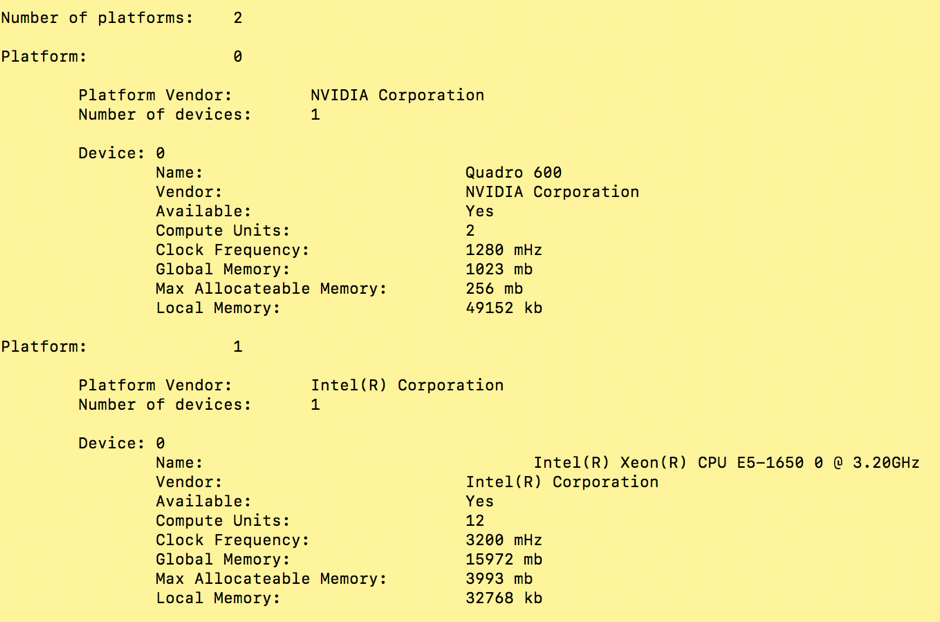
\includegraphics[width=11cm]{figures/Devquery.png}
\caption{Device characterisitcs of Intel Xeon E5-1650 CPU and NVIDIA Quadro 600 CPU}
\label{fig:cnn17}
\end{figure}

Because of the higher number of compute units (12) for the CPU, OpenCL brings about parrallelisation of the code to a much greater extent, as compared to the GPU (2). Furthermore, the clock frequency at which the CPU can execute at (3.2 GHz) is higher than that of  the GPU (1.28 GHz). Thus, this CPU shows better performance relative to the GPU in executing OpenCL kernels.
\chapter{RISC-V}
\label{ch6_riscv}

\section{Introduction}
 \label{sect6_1}
 
The performance derived from a computer and the amount of energy that is consumed in the process hugely depends on algorithms, application code, compiler, microarchitecture, Instruction Set Architecture (ISA), physical design, circuit design and fabrication process. This is the order of abstraction from a user working on the computer, starting from the top most layer exposed to programmer, down to the bottom most layer which depends on how the chip is fabricated. \newline\newline
The Central Processing Unit (CPU) is one of the most significant parts of any computing device, as it is the brain of the computer [12]. It performs arithmetic and logical operations and moves data from one place to another. This is done by the processor according to ISA it is based on. An ISA is a well-defined interface linking computer software to the hardware its running on, enabling the independent development of the two computing realms. It is strictly an interface specification, not an implementation. \newline\newline
In today’s age, technology has been able to evolve much more because of the existence of open standards and open source software – Linux as an open source operating system for example. This builds the case for an ISA which is not proprietary and is powerful enough to drive custom processing chips. \newline\newline
Historically, ISAs have been proprietary for business reasons, but there is no good technical reason for the absence or deficiency of open source ISAs. Having a free and open source ISA specification would hugely benefit the industry, just like how open source software has added great value. It would directly lead to a rise in innovation via free-market competition, with several designers coming with various implementations, which comprise both the open source and proprietary ISA versions. More shared open core designs would exist, reducing the time taken to hit the market, lowering cost from reuse, and making the designs more transparent and error-free. Moreover, an open ISA would lead to processors becoming affordable for a greater number of devices, helping in expanding the Internet of Things (IoTs) [13].

\subsection{About}
 \label{sect6_1_1}
RISC-V is an ISA originally designed to support computer architecture research and education, now reaching the stage to become a standard open architecture for industry implementations, under the governance of the RISC-V foundation. It was developed in the Computer Science Division of the EECS department at University of California, Berkeley [14]. Its development was inspired by ARM’s IP restrictions together with the lack of 64-bit addresses. \newline\newline
RISC-V has learned from various mistakes in different ISAs, making its design superior to other ISAs incorporating a better mix of capabilities [13]. It provides a small core instruction set that compilers and operating systems can depend on, as well as optional standard extensions. It has a compact instruction set encoding – smaller code is desirable as it reduces the memory requirement. It offers single, double and quadruple precision floating point capabilities, in addition to being 32, 64 and 128-bit addressable. \newline\newline
RISC-V was defined with a goal to be completely open and freely open to academic researchers and industries. Designed with small, fast and low-power real-word implementations in mind, it does not over-architect for a particular style of microarchitecture. It is a real ISA suited for direct native hardware implementation, not for just simulation or binary translation. It provides support for the revised 2008 IEEE-754 floating-point standard [15]. RISC-V simplifies experiments with new supervisor-level and hypervisor-level ISA designs. \newline\newline
RISC-V’s capabilities make it extremely powerful, yet simple and clean to implement. In contrast to most ISAs, it is available for all types for use, empowering anyone to design, manufacture and sell RISC-V chips and software. It supports small embedded systems, Personal Computers (PCs), supercomputers with vector processors, and warehouse-scale rack mounted parallel computers. Thus, the widespread usage of RISC-V would allow software developers to target an open hardware target, while making commercial processor designers compete on implementation superiority. 

\subsection{ISA Specifications}
 \label{sect6_1_2}
RISC-V is specified as a base integer ISA, which is a must in any implementation, with additional extensions to the base ISA. Based on the width of the integer registers, the base instruction set has two variants, RV32I and RV64I. There is scope for a future variant RV128I for 128-bit address support. [16] It provides support for extensive customization and specialization, along with extension beyond the base instruction set, but doesn’t allow redefining these base integer instructions. \newline\newline
There are four core instruction formats defined in the base instruction set, as shown follows:
\begin{figure}[h!]
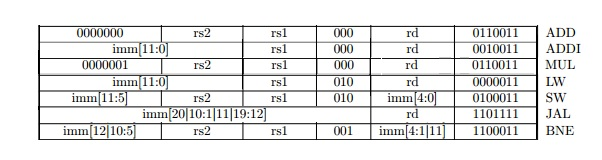
\includegraphics[width=\linewidth]{figures/RISCV_Instruction_Formats.jpg}
\caption{Base instruction formats in RISC-V}
\label{fig:riscv1}
\end{figure}

Furthermore, there are two variations of the instruction formats (SB/UJ) based on how immediate values are taken care of. A few sets of standard extensions have been pre-defined to cater to general software development. These comprise integer multiplication/division (extension “M”), atomic operations (extension “A”), single-precision floating-point (extension “F”), and double-precision floating-point (extension “D”). A combination of these 4 standard extensions (denoted by “IMAFD”) is given a general abbreviation of “G”, which results in a general-purpose scalar instruction set. RV32G and RV64G are currently set as default targets of the RISC-V compiler toolchains. The base set and extensions have been kept separated to have a simple instruction set. \newline\newline
The base integer instruction set for the 32-bit and 64-bit variants (RV32I/RV64I) comprises 40 instructions, while the general-purpose instruction set (RV32G/RV64G) supports 122 instructions. There are 31 general purpose registers x1-x31 capable of storing integer values, register x0 being hardwired to the constant value 0. The register width is 32 bits for RV32I and 64 bits for RV64I. RISC-V is based on the load-store architecture, where arithmetic operations only function on the data stored the registers and only the load and store operations access memory. The user address space is byte-addressed and little-endian. \newline\newline
There also exists a reduced version of the base integer instruction set (RV32I), designed specifically for embedded systems (denoted by “E”). The major difference is that the number of registers in RV [17]32E is reduced to 16 from 31 in RV32I. A draft proposal for the RISC-V standard compressed instruction set has been made which reduces static and dynamic code size by adding short 16-bit instruction encodings for conventional operations. Denoted by the extension “C”, it could be added to any of the base ISA variants (RV32I, RV64I, and RV128I). 

 \section{Software Tools and Setup Required}
  \label{sect6_2}

\subsection{Software Tools}
 \label{sect6_2_1}
Several software tools and libraries are required to be downloaded and setup before any development on RISC-V can begin. These comprise the riscv-tools infrastructure and are available on GitHub. It is a meta-repository with Git submodules containing every stable component of the RISC-V software toolchain [18]. The image below shows the software stack of riscv-tools: \newline\newline
\begin{figure}[h!]
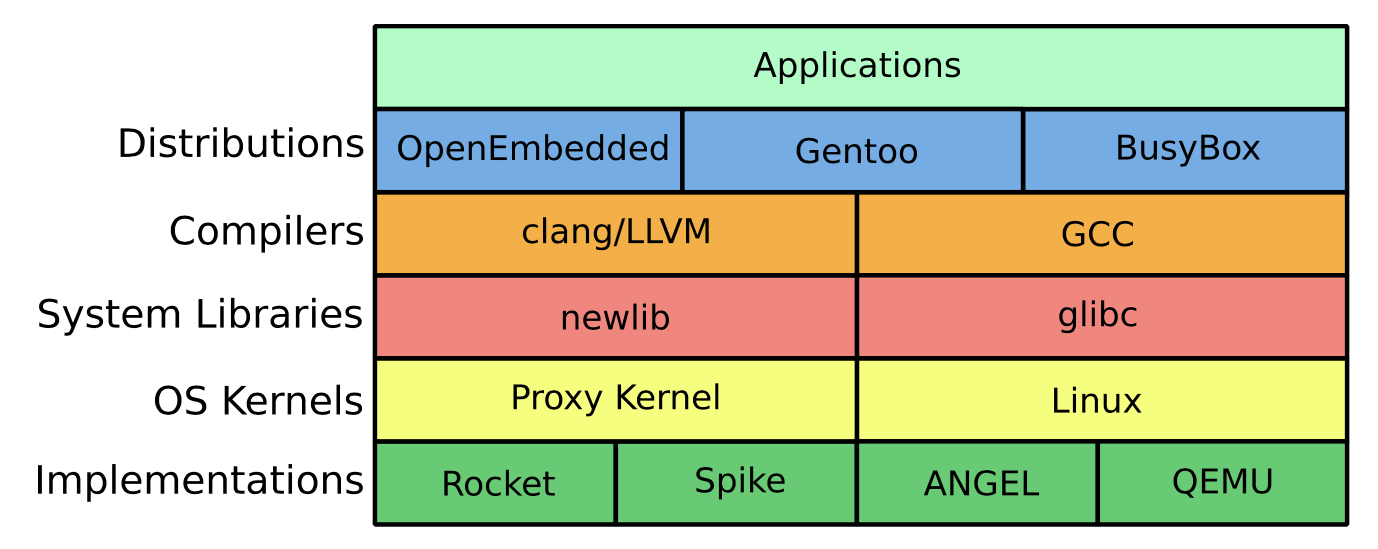
\includegraphics[width=\linewidth]{figures/RISC-V_Software_Stack.png}
\caption{Software stack for RISC-V tools}
\label{fig:riscv2}
\end{figure}

\subsubsection{GNU Toolchain}
 \label{sect6_2_1_1}
The RISC-V GNU Toolchain is a RISC-V C and C++ cross compiler utility. It contents include binutils, gcc, newlib, glibc, and Linux UAPI headers. It supports two build modes: a generic ELD/Newlib toolchain and a more sophisticated Linux-ELF/glibc toolchain. The riscv-unknown-elf command is used to compile a program while riscv64-unknown-elf-gcc is used to assemble and link with gcc/binutils.

\subsubsection{Front End Server}
 \label{sect6_2_1_2}
RISC-V front end server library facilitates communication between the host machine and the RISC-V target device on the Host-Target Interface (HTIF). It also provides a virtualized console and disk device [19]. 

\subsubsection{Proxy Kernel}
 \label{sect6_2_1_3}
RISC-V proxy kernel is responsible for servicing system calls generated by code built and linked with the RISC-V Newlib port [19]. It handles system calls like open, close and printf. Abbreviated as \verb|pk| (or \verb|riscv-pk|), it is a lightweight application execution environment that can host statically-linked RISC-V ELF binaries. It is designed to support tethered RISC-V implementations with limited I/O capability and thus handles I/O-related system calls by proxying them to a host computer [20].

\subsubsection{ISA Simulator}
 \label{sect6_2_1_4}
RISC-V ISA simulator consists of a functional simulator known as Spike [19]. It implements a functional model of one or more RISC-V processors [21]. Since there is no proper operating system, it executes the generated binary running on top of the proxy kernel. \newline\newline
Spike takes the path of the binary to run as its argument, which is \verb|pk|, located at \verb|$RISCV/riscv-elf/bin/pk| and finds it automatically. The name of the program to be run is the argument for \verb|riscv-pk|, which then executes the program. An interactive debug mode can be invoked in Spike with the -d command line flag or \verb|SIGINT|, which enables single-stepping through instructions, setting break point conditions, printing register and memory contents, etc.

\subsubsection{Opcodes}
 \label{sect6_2_1_5}
RISC-V Opcodes is a subcomponent of riscv-tools which enumerates all standard RISC-V instruction opcodes executable by the simulator, and control and status registers (CSRs). It also has a script to convert them into different formats (C, Scala, LaTex) [22].

\subsection{Setup Required}
 \label{sect6_2_2}
There are many possible combinations to pick for the different layers of the stack shown in Figure 4, but there exist 2 of the most common workflows for RISC-V software development [18]. These are as follows:
\begin{itemize}
\item \textbf{Spike + pk} \newline
The use case for following this workflow are embedded or single applications.
\begin{itemize}
\item Distributions: None
\item Compilers: clang/LLVM or GCC
\item System Libraries: newlib
\item OS Kernels: Proxy Kernel (pk)
\item Implementations: Spike
\end{itemize}	
	
\item \textbf{QEMU + Linux} \newline
The use case for following this workflow is Simple POSIX environment.
\begin{itemize}
\item Distributions: BusyBox
\item Compilers: GCC
\item System Libraries: glibc
\item OS Kernels: Linux
\item Implementations: QEMU
\end{itemize}
\end{itemize}
In this case, the former workflow was followed, the aim being familiarization with the RISC-V development phase. The selected workflow was easier to set up and took lesser time. This requires the components riscv-gnu-toolchain, riscv-fesvr, riscv-isa-sim, and riscv-pk. \newline\newline
The binaries generated against newlib system library will not be running on a full-blown operating system, but will require access to few crucial system calls [19]. The setup will thus require the installation of riscv-newlib. Newlib is a C library intended for embedded systems. It has the edge of not being unnecessarily complicated over Glibc, as well as having sufficient support. Also, its porting process is much simpler than that of Glibc because it only requires a few stubs of glue code. These stubs of code include the system calls that are supposed to call into the operating system you’re running on.

\subsubsection{Toolchain}
\label{sect6_2_2_1}
The following steps were followed to obtain and compile the RISC-V toolchain sources for the above-mentioned workflow:
\begin{enumerate}
\item To build GCC, several other Ubuntu packages like \verb|flex|, \verb|bison|, \verb|autotools|, \verb|libmpc|, \verb|libmpfr|, and \verb|libgmp| are required. Obtain the required Ubuntu packages required for installation with this command:\newline
\small \textbf{sudo apt-get install autoconf automake autotools-dev curl libmpc-dev libmpfr-dev libgmp-dev gawk build-essential bison flex texinfo gperf libtool patchutils bc}

\item Set the environment variables \verb|TOP| as the directory where the tools will be installed, i.e. the current working directory:\newline
\small \textbf{export \$TOP = \$(pwd)}

\item Clone riscv-tools repository from GitHub:\newline
\small \textbf{git clone https://github.com/riscv/riscv-tools.git}

\item Change into the \verb|riscv-tools| directory:\newline
\small \textbf{cd \$TOP/riscv-tools}

\item Instruct Git to update its submodules:\newline
\small \textbf{git submodule update –--init --recursive}

\item Set the \verb|RISCV| environment variable to point to the path where new tools will be installed:\newline
\small \textbf{export \$RISCV = \$TOP/riscv}

\item The \verb|PATH| environment variable also needs to be set to point to the directory specified by RISCV:\newline
\small \textbf{export \$PATH = \$PATH:\$RISCV/bin}

\item After everything has been set up, run the \verb|build| script:\newline
\small \textbf{./build.sh}
\end{enumerate}

A successful build marks the end of the toolchain installation process.

\subsubsection{Testing}
\label{sect6_2_2_2}
After the installation procedure is finished, testing was done to make sure that there were no issues with the set up. 
\begin{enumerate}
\item Change to the directory of toolchain installation:\newline
\small \textbf{cd \$TOP}
\item Write a simple “Hello World” program in a C file
%\small \textbf{echo \–e }\#include <stdio.h> '\n' int main(void) { printf(“Hello world!”); return 0; }’ \> hello.c
\item Build your program using the \verb|riscv64-unknown-elf-gcc| command:\newline
\small \textbf{riscv64-unknown-elf-gcc -o hello hello.c}
\item Run the binary on the ISA Simulator (Spike):\newline
\small \textbf{spike pk hello}
\end{enumerate}

The output generated should be "Hello world!", as shown below in Figure \ref{fig:riscv3} \newline

\begin{figure}[h!]
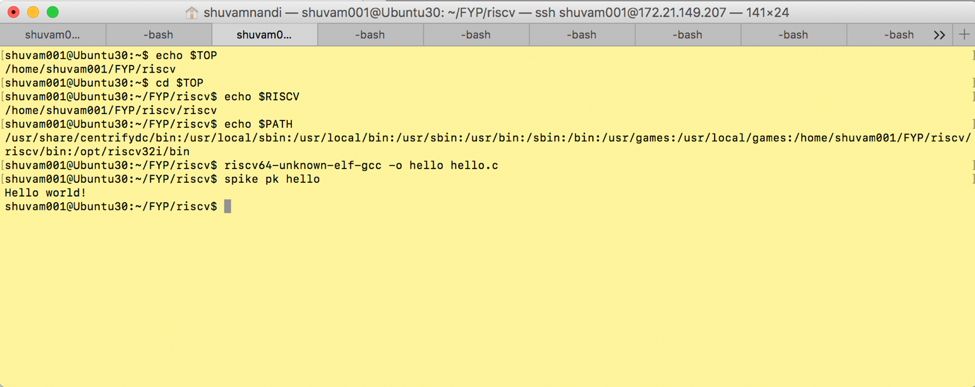
\includegraphics[width=\linewidth]{figures/Spike_Output.png}
\caption{Hello World program execution on Spike}
\label{fig:riscv3}
\end{figure}

 \section{PicoRV32}
  \label{sect6_3}
To understand how RISC-V is implemented in real, a processor implementation PicoRV32 was studied and analyzed. PicoRV32 is a processor core implementing the RV32IMC instruction set. It can be configured as RV32E, RV32I, RV32M, RV32C, or RV32IMC, and optionally contains a built-in interrupt controller. It is available free and is open sourced under the ISC license [17]. 

\subsection{About}
 \label{sect6_3_1}
PicoRV32 is a small sized processor which can operate at high frequencies (250-450 MHz on 7-Series Xilinx FPGAs). The core exists in two variants, \verb|picorv32| and \verb|picorv32_axi|. The former providing a simple native memory interface, easy to use in simple environments, while the latter providing an AXI-4 Lite Master interface that can be easily integrated with existing systems already using the AXI standard. It provides a selectable native memory interface, optional IRQ support and optional co-processor interface. This CPU core is designed to be added as an auxiliary processor in FPGA designs and ASICs. It could be easily integrated with most existing designs without exceeding clock domains. 

\subsection{Setup Required}
 \label{sect6_3_2}
PicoRV32 is based on the 32-bit version of RISC-V ISA, hence requires a setup of the complete toolchain targeting a pure RV32I CPU. 

\subsubsection{Toolchain}
 \label{sect6_3_2_1}
The following steps will download the toolchain required for programs to be compiled on PicoRV32 processor:

\begin{enumerate}
\item To build GCC, several other Ubuntu packages like \verb|flex|, \verb|bison|, \verb|autotools|, \verb|libmpc|, \verb|libmpfr|, and \verb|libgmp| are required. Obtain the required Ubuntu packages required for installation with this command:\newline
\small \textbf{sudo apt-get install autoconf automake autotools-dev curl libmpc-dev libmpfr-dev libgmp-dev gawk build-essential bison flex texinfo gperf libtool patchutils bc}

\item Create a new directory \verb|/opt/riscv32i| to store the toolchain once installed:
\newline
\small \textbf{sudo mkdir /opt/riscv32i}

\item Change permissions of the directory created in the previous step:\newline
\small \textbf{sudo chown \$USER /opt/riscv32i}

\item Obtain the toolchain from the riscv-tools GitHub repository of RISC-V foundation and store it in the directory \verb|riscv-gnu-toolchain-rv32i|:\newline
\small \textbf{git clone https://github.com/riscv/riscv-gnu-toolchain riscv-gnu-toolchain-rv32i}

\item Change into this directory:
\newline
\small \textbf{cd riscv-gnu-toolchain-rv32i}

\item Checkout the specific commit version:
\newline
\small \textbf{git checkout 914224e}

\item Update submodules within the repository:
\newline
\small \textbf{git submodule update --init --recursive}


\item Create a new directory \verb|build|:
\newline
\small \textbf{mkdir build}

\item Change into this directory:
\newline
\small \textbf{cd build}

\item Run the \verb|configure| script, which specifies the instruction set architecture as RV32I, and the directory to install the toolchain as /opt/riscv32i:
\newline
\small \textbf{../configure --with-arch=rv32i --prefix=/opt/riscv32i}

\item Run the \verb|make| script to build the toolchain:
\newline
\small \textbf{make -j\$(nproc)}
\end{enumerate}

\subsubsection{PicoRV32 Source Code}
 \label{sect6_3_2_2}
Now that the pure RV32I toolchain is downloaded, the CPU implementation can be downloaded and tested.

\begin{enumerate}
\item Clone PicoRV32 repository from GitHub:\newline
\small \textbf{git clone https://github.com/cliffordwolf/picorv32.git}

\item Run the \verb|make| script to build the toolchain:\newline
\small \textbf{cd \texttildelow /picorv32}

\item Run the \verb|make| script in the PicoRV32 source directory to download RV32IMC toolchains to be able to run all tests:\newline
\small \textbf{make -j\$(nproc) build-riscv32imc-tools - RV32IMC}

\end{enumerate}

\subsubsection{Icarus Verilog}
\label{sect6_3_2_3}
In order to test the working of the downloaded toolchain, the test bench provided by PicoRV32 must be run. This requires a software called \textit{Icarus Verilog}, which needs to be installed. Icarus Verilog is a Verilog simulation and synthesis tool. It operates as a compiler, compiling source code written in Verilog (IEEE-1364) into some target format. For batch simulation, the compiler can generate an intermediate form calledvvp assembly. This intermediate form is executed by the vvp command. For synthesis, the compiler generates netlists in the desired format [23]. The following steps will download and install Icarus Verilog:

\begin{enumerate}
\item Clone the GitHub repository:\newline
\small \textbf{git clone https://github.com/steveicarus/iverilog.git}

\item Change into the \verb|iverilog| directory:\newline
\small \textbf{cd iverilog}

\item Update to the latest code in master branch:\newline
\small \textbf{git pull origin master}

\item Install \verb|autoconf| and \verb|gperf| packages installed for the configuration script to work (skip if step already done):\newline
\small \textbf{sudo apt-get install autoconf gperf}

\item Run \verb|autoconf.sh| script:\newline
\small \textbf{sh autoconf.sh}

\item Run \verb|configure| script:\newline
\small \textbf{./configure}

\item Run \verb|make| command with sudo access:\newline
\small \textbf{sudo make}

\item Run \verb|make| install:\newline
\small \textbf{make install}
\end{enumerate}

\subsection{Execution of Simple C Programs}
 \label{sect6_3_3}
After the installation of all tools required for using PicoRV32 was completed, the testbench provided was run by executing the make command. The following output was obtained:\newline\newline

\begin{figure}[h!]
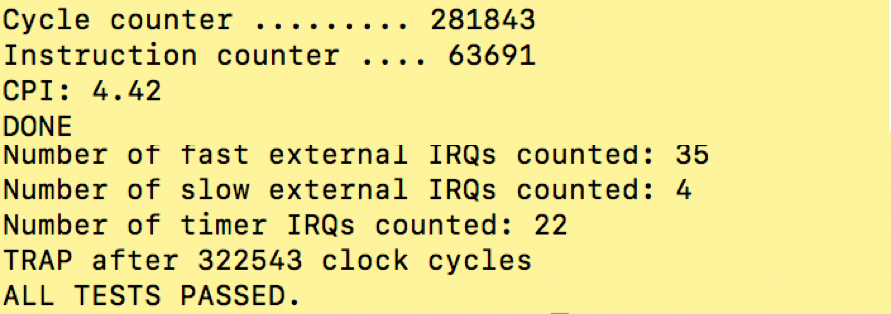
\includegraphics[width=\linewidth]{figures/PicoRV32_Execution.png}
\caption{Successful execution of PicRV32 testbench}
\label{fig:riscv4}

\end{figure}

This demonstrates that the installation was done successfully. The output is produced by different C files which are executed on the PicoRV32 CPU. The functions written in the C files are called in an assembly file \textit{start.S}, located in \verb|picorv32/firmware| directory. Along with C function calls, the assembly file also contains various tests in assembly files which get executed upon running make command. \newline\newline
Upon further analysis of the compilation and execution flow, it was observed that the Icarus Verilog compiler compiles the \textit{testbench.v} and \textit{picorv32.v} files and generates an intermediate \verb|vvp| assembly file, \textit{testbench.vvp}. This is followed by the compilation of the \textit{start.S} assembly file, the C codes and test assembly files the into their binaries using the \verb|riscv32-unknown-elf-gcc| command. This is succeeded by the generation of an executable file \textit{firmware.elf}, which is translated into a \textit{firmware.bin} file by \verb|riscv32-unknown-elf-objcopy| utility. In order to run the machine code on the processor, a script makehex.py in the firmware directory was used to convert the \textit{firmware.elf} file into \textit{firmware.hex} file. The \textit{firmware.hex} file contains instructions as defined by the RISC-V specification in the 32-bit format (represented as 8 digit hexadecimal numbers), which are passed to PicoRV32. The \verb|vvp| command of Icarus Verilog runs the previously generated \textit{testbench.vvp} file and executes the machine code on PicoRV32. \newline\newline
Observing the testbench output provided deep insights into how the execution maps from the high-level language C code to the low-level machine code. To understand how the processor executes these instructions, the Verilog file \textit{picorv32.v} was studied and understood. The instructions are loaded from the firmware.hex file in the testbench, which is stored in a 1024-bit wide register. \newline\newline
The above code snippet shows the loading of the instructions into a 32-bit wide, 16384 lines long memory in an \verb|axi4_memory| instance. The instance is declared as follows: \newline\newline
This memory is the source of instructions for the processor, which lacks a default instruction memory. As mentioned in 5.3.1, PicoRV32 is available in two variants. In this case, the \verb|axi4_memory| is interfaced to the \verb|picorv32_axi| version of PicoRV32 core, using the \verb|picorv32_axi_adapter|.

 \section{Implementation of RISC-V Processor}
 \label{sect6_4}
After understanding the working of PicoRV32 from a high-level perspective, the next step is to design and implement a small processor based on the RISC-V 32-bit base integer instruction set. PicoRV32 has several features, like custom instructions for IRQ handling, which make the processor complicated, heavier and relatively slower. 
On an average, PicoRV32 was observed to have a Cycles Per Instruction (CPI) value of 4.8. The execution of some specific instructions increased the CPI. 

\subsection{Objective}
\label{sect6_4_1}
The objective is to develop a smaller and more efficient processor and analyze whether it could perform better than PicoRV32. The initial implementation intends to be capable of performing only a small set of instructions and compare its performance with PicoRV32. A fully functional processor implementing RISC-V ISA meeting the desired requirements (as mentioned in Section 6.4.2) must be developed before it could be further extended. 

\subsection{Design}
\label{sect6_4_2}
\subsubsection{Requirements}
\label{section:sect6_4_2_1}
The design of any RISC based processor follows the load store architecture. It would be a 32-bit variant of the base integer instruction set, meaning that the registers width would be 32 bits. To start off with, the following instructions need to be present in our RISC-V implementation:
\begin{itemize}
\item Arithmetic: ADD, ADDI, MUL
\item Load/Store: LW, SW
\item Jump: JAL
\item Branch: BNE
\end{itemize}
Among the above instructions, ADD, MUL, fall into the category of R-type instructions; ADDI and LW fall into the I-type instruction category, SW is in the S-type instruction category; JAL is in the UJ-type instruction category; BNE uses the SB-type instruction format. \newline\newline
Harvard architecture is selected over von Neumann architecture, as data and instruction memory separation is preferred. Two separate memory systems can perform better than having a single, unified memory for both data and instructions. The various components required by the processor implementation would be the control unit, registers, Arithmetic and Logic Unit (ALU) and instruction memory.

\subsubsection{Components}
\label{sect6_4_2_2}
The processor would be built using the required components as stated above in \ref{section:sect6_4_2_1}. This section discusses the functional requirements desired in the components.

\begin{enumerate}
\item \textbf{Control Unit} \newline
The Control Unit determines the execution of operations on the processor. It instructs the processor’s components like memory, ALU and input and output devices to respond to the program instructions. It can be perceived as the brain inside the CPU, making it the brain inside the brain of the computer. \newline\newline
It consists of two registers, namely the Program Counter (PC) register and the Instruction Register (IR). PC points to the address of the instruction to be executed, while IR contains the instruction being currently interpreted. Instructions are fetched from the instruction memory and decoded in the Control Unit. The data required for the instruction to execute is extracted from the registers or data memory, and passed on to the ALU to perform the operation specified by the instruction opcode. \newline\newline
The design of the control unit needs to be done according to RISC-V instruction specifications. As seen in Figure \ref{fig:riscv5}, the instruction contains additional information about the instruction in bits func7 and func3 which distinguish several instructions; opcodes can be the same for various instructions, as shown below.

\begin{figure}[h!]
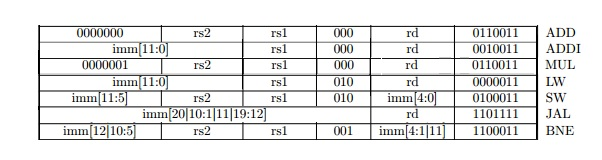
\includegraphics[width=\linewidth]{figures/RISCV_Instruction_Formats.jpg}
\caption{Formats for RISC-V instructions to be implemented}
\label{fig:riscv5}
\end{figure}

\item \textbf{Registers} \newline
Under the RISC-V specification, the base integer instruction set has a set of 32 registers, each 32-bit wide (x1-x31, x0 hardwired to constant 0). The Control Unit decodes instructions and extracts the register address on which the ALU needs to perform specified instructions. Data can be transferred between memory and registers using the load and store instructions. Thus, in a load store architecture, register memory is significant and should be wisely used in order to reduce overheads of memory accesses. It can be declared as shown in the following code snippet:

\item \textbf{Memory} \newline
Memory stores instructions and data. Being a Harvard Architecture processor, there would be a clear separation of instructions and data. A little endian memory system would be followed. The instruction memory stores the instructions generated by the makehex.py script, converting the firmware.bin file to firmware.hex format. The width and length of the instruction memory are 32 bits and 16384 lines, respectively. 

\item \textbf{Arithmetic and Logic Unit} \newline
The Arithmetic and Logic Unit of a CPU performs arithmetic and logical operations on operands specified by the instructions. It is the fundamental unit of the CPU of any computing device. After performing an operation, the result is stored back into the register file at the address specified by the instruction.

\begin{figure}
\centering
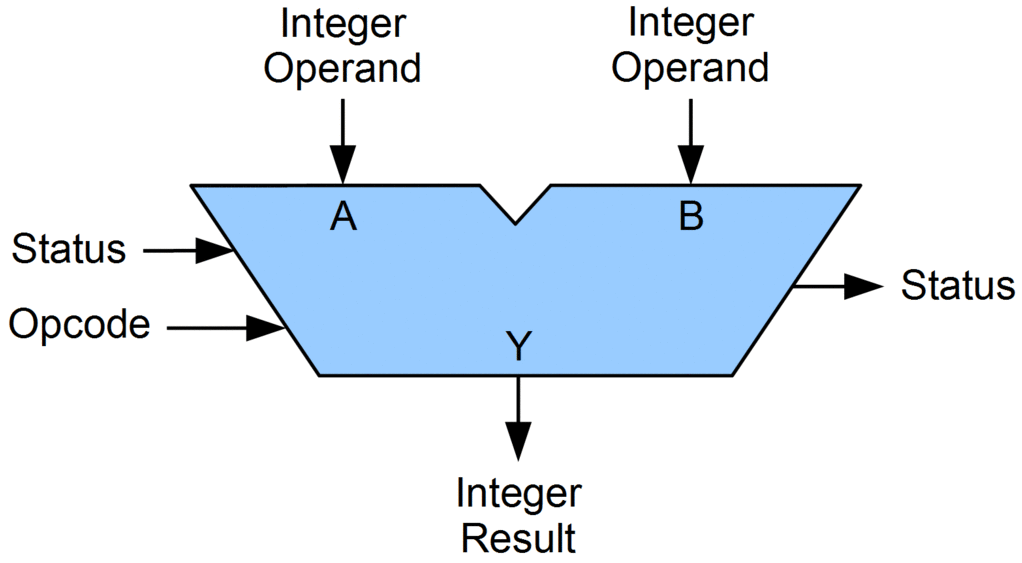
\includegraphics[width=8.5cm]{figures/ALU_block.PNG}
\caption{Symbolic representation of an ALU}
\label{fig:riscv6}
\end{figure}

\end{enumerate}






\chapter{Conclusions and Future Work}
\label{ch7_conclusion}
This chapter concludes and summarizes this report.
Furthermore, in this chapter we discuss future research directions in detail.

\section{Conclusions}

\section{Future work}



\begin{appendices}
	
\chapter{CNN}
\lstset { %
	language=C,
	backgroundcolor=\color{white},
	basicstyle=\ttfamily\tiny,
	keywordstyle=\color{magenta}\ttfamily,
	stringstyle=\color{blue}\ttfamily,
	commentstyle=\color{green}\ttfamily,
    breakatwhitespace=false,
	breaklines=true	
}
\lstset{framesep=-5pt, xleftmargin=-5pt}

\begin{table}[!h]
\centering
\caption{Model of LeNet-5 Layers }
\label{cnncode1:lenet5}
\begin{tabular}{l}
\toprule
\begin{lstlisting}[columns=fullflexible, language=C]
#ifndef _LENET5_MODEL_H_
#define _LENET5_MODEL_H_
#include <stdio.h>

#define CONV1_NO_INPUTS  1
#define CONV1_NO_OUTPUTS  20
#define CONV1_FILTER_HEIGHT  5
#define CONV1_FILTER_WIDTH  5

extern const float conv1_weights[CONV1_NO_OUTPUTS][CONV1_NO_INPUTS*CONV1_FILTER_HEIGHT*CONV1_FILTER_WIDTH];
extern const float conv1_bias[CONV1_NO_OUTPUTS];

#define CONV2_NO_INPUTS  20
#define CONV2_NO_OUTPUTS  50
#define CONV2_FILTER_HEIGHT  5
#define CONV2_FILTER_WIDTH  5

extern const float conv2_weights[CONV2_NO_OUTPUTS][CONV2_NO_INPUTS*CONV2_FILTER_HEIGHT*CONV2_FILTER_WIDTH];
extern const float conv2_bias[CONV2_NO_OUTPUTS];

#define IP1_NO_INPUTS  800
#define IP1_NO_OUTPUTS  500

extern const float ip1_weights[IP1_NO_OUTPUTS][IP1_NO_INPUTS];
extern const float ip1_bias[IP1_NO_OUTPUTS];

#define IP2_NO_INPUTS  500
#define IP2_NO_OUTPUTS  10

extern const float ip2_weights[IP2_NO_OUTPUTS][IP2_NO_INPUTS];
extern const float ip2_bias[IP2_NO_OUTPUTS];

#endif // _LENET5_MODEL_H_
\end{lstlisting}
\\
\bottomrule
\end{tabular}
\end{table}

	
\chapter{RISC-V}
\lstset { %
	language=Verilog,
	backgroundcolor=\color{white}, % set backgroundcolor
	%basicstyle=\footnotesize,% basic font setting
	%basicstyle=\ttfamily\tiny,
	basicstyle=\ttfamily\tiny,
	keywordstyle=\color{blue}\ttfamily,
	stringstyle=\color{red}\ttfamily,
	commentstyle=\color{green}\ttfamily,
    breakatwhitespace=false,
	breaklines=true	
}
\lstset{framesep=-10pt, xleftmargin=-10pt}

\begin{table}[!h]
\centering
\caption{RISC-V Processor Testbench}
\label{riscvcode1:tb}
\begin{tabular}{l}
\toprule
\begin{lstlisting}[columns=fullflexible, language=Verilog]
module testbench_rvproc;

	// Inputs
	reg clk;
	reg rst;
	reg [`ISIZE-1:0] addr; 

	// Outputs
	wire [`DSIZE-1:0] instr_out;

	rvproc uut (
		.clk(clk), 
		.rst(rst), 
		.PCOUT(addr), 
		.instr_out(instr_out));
        
	always #5 clk = ~clk;
	initial 
	  begin
	  // Initialize Inputs
	  clk = 0;
          rst = 1;
	  addr = 32'h0000_0000;
      
	  // Wait 20 ns for global reset to finish
          #20;
          
	  // Add stimulus here
	  rst = 0;
	  addr = 32'h0000_0000;
	end	
endmodule
\end{lstlisting}
\\
\bottomrule
\end{tabular}
\end{table}

\begin{table}[!h]
\centering
\caption{RISC-V Processor Program Counter and Control Unit}
\label{riscvcode2:pc_cu}
\begin{tabular}{l}
\toprule
\begin{lstlisting}[columns=fullflexible, language=Verilog]
module program_counter(input clk, input rst, input [`ISIZE - 1:0]nextPC, 
output reg [`ISIZE - 1:0]currPC);
  always @( posedge clk)
  begin
      if (rst) begin  currPC <= 16'h0000; end
      else begin currPC <= nextPC; end
  end
endmodule
\end{lstlisting}
\\
\midrule

\begin{lstlisting}[columns=fullflexible, language=Verilog]
module control(input reg [3:0] instr_code, output reg wen, output reg mem_read, 
output reg mem_write, output reg AluToReg, output reg branch, output reg jr, output reg jal);  
  initial
  begin
	wen = 0; mem_read = 0; mem_write = 0; AluToReg = 1;
	branch=0;jr=0;jal=0;
  end  
  always@(*)
 	 begin
		wen = 1; mem_read = 0; mem_write = 0; AluToReg = 1;
		branch = 0;	jr=0; jal=0;
		case(instr_code)
			`LW: begin
				mem_read = 1;
				AluToReg = 0;
			end
			`SW: begin
				wen = 0;
				mem_write = 1;
			end
			`JR: begin
				wen = 0;
				jr = 1;
			end
			`JAL: begin
				wen = 0;
				jr = 1;	jal = 1;
			end
			`BNE: begin
				wen = 0;
				branch = 1;
			end
		endcase
	end
endmodule
\end{lstlisting}
\\
\bottomrule
\end{tabular}
\end{table}

\begin{table}[!h]
\centering
\caption{RISC-V Processor Decoder}
\label{riscvcode3:dec}
\begin{tabular}{l}
\toprule
\begin{lstlisting}[columns=fullflexible, language=Verilog]
module decoder(
    input [`ISIZE-1:0] instr,  //32-bit instruction	
    output reg [3:0] instr_code, //Instruction code
    output reg [`ASIZE-1:0] rs1,    //Source Register address 1
    output reg [`ASIZE-1:0] rs2,    //Source Register address 2
    output reg [`ASIZE-1:0] rd,     //Destination Register address
    output reg [`DSIZE-1:0] imm    //Sign extended immediate value
    );
 
    always @(*)
    begin        
        case(instr[6:0])

          `RTYPE_OPC: begin
              rs1 = instr[19:15];
              rs2 = instr[24:20];
              rd = instr[11:7];
              case(instr[31:25])        //ADD MORE CASES HERE FOR SUB, SRA
                7'b0000000: begin
                  case(instr[14:12])    //ADD MORE CASES HERE FOR AND, OR, XOR, SLT, SLTU, SRL, SLL
                    3'b000: instr_code = `ADD;    
		  endcase
                end
                7'b0000001: instr_code = `MUL;
              endcase
          end

          `ITYPE_OPC: begin
              rs1 = instr[19:15];
              imm={{20{instr[31]}}, {{instr[31:20]}}};
              rd = instr[11:7];
              case(instr[14:12])
                3'b000: instr_code = `ADDI;
              endcase
          end

          `LW_OPC: begin
            rs1 = instr[19:15];
            imm={{20{instr[31]}}, {{instr[31:20]}}};
            rd = instr[11:7];
            instr_code = `LW;
          end

    		  `SW_OPC: begin
            rs1 = instr[19:15];
            rs2 = instr[24:20];
            imm={{20{instr[31]}}, {{{{instr[31:25]}, {instr[11:7]}}}}};
            instr_code = `SW;
          end
          `JAL_OPC: begin //NOT COMPLETE
            rd = instr[11:7];
            imm={{12{instr[31]}}, {{instr[31:12]}}};
            instr_code = `JAL;
          end
          
          `JR_OPC: begin
            rs1 = instr[19:15];
            instr_code = `JR;
          end
          
    		  `CONBRANCH_OPC: begin
            rs1 = instr[19:15];
            rs2 = instr[24:20];
            imm={{21{instr[31]}}, {{{{instr[7]}, {instr[30:25]}, {instr[11:8]}}}}};
            case(instr[14:12])
              3'b001: instr_code = `BNE;
            endcase
          end
        endcase
    end
endmodule
\end{lstlisting}
\\
\bottomrule
\end{tabular}
\end{table}
\begin{table}[!h]
\centering
\caption{RISC-V Processor ALU and Register file}
\label{riscvcode4:alu_reg}
\begin{tabular}{l}
\toprule

\begin{lstlisting}[columns=fullflexible, language=Verilog]
module alu(
    clk, rst, instr_code,
    a,   //1st operand
    b,   //2nd operand
    imm, //32 bit immediate value
    out,   //output
  	zero   //zer flag bit for branch 
    );
    input clk, rst;
    input[3:0] instr_code;
    input [`DSIZE-1:0] a, b, imm;
    output reg [`DSIZE-1:0] out;
    output reg zero;      
    always @ * 
    begin
      case(instr_code)
        `ADD: out = a + b;
        `MUL: out = a * b;
        `ADDI: out = a + imm;
        `LW: out = a + imm;
        `SW: out = a +imm;
        `BNE: out = a - b;
      endcase    	
    	if(out==0)
    		zero=1;
    	else
    		zero=0;
    end
endmodule
\end{lstlisting}
\\
\midrule

\begin{lstlisting}[columns=fullflexible, language=Verilog]
module regfile (input clk, input rst, input write_en, input [`ASIZE-1:0] raddr1, input [`ASIZE-1:0] raddr2, 
	input [`ASIZE-1:0] waddr, input [`DSIZE-1:0] wdata, output [`DSIZE-1:0] rdata1, 
    output [`DSIZE-1:0] rdata2);

	reg [`DSIZE-1:0] regdata [0:`NREG-1];
	
	integer i;
	initial begin
		for (i = 0; i < `NREG; i = i+1)
			regdata[i] = 0;
	end

	always@(posedge clk)
		begin
			if(rst)
				begin
					for (i=0; i<`NREG; i=i+1)
						regdata[i] <=0;
					regdata[1] <=1;//initialization regdata[1] is initialized with 1.
					regdata[2] <=1;//initialization regdata[2] is initialized with 1.
					regdata[3] <=4;//initialization regdata[3] is initialized with 4.
					regdata[4] <=3;//initialization regdata[4] is initialized with 3.
					regdata[5] <=2;//initialization regdata[5] is initialized with 2.
					regdata[6] <=1;//initialization regdata[6] is initialized with 1.
					regdata[7] <=6;//initialization regdata[7] is initialized with 6.
					regdata[8] <=4;//initialization regdata[8] is initialized with 4.
					regdata[9] <=2;//initialization regdata[9] is initialized with 2.					
				end
			else
				regdata[waddr] <= ((write_en == 1)) ? wdata : regdata[waddr];
		end
	assign rdata1 = ((write_en) && (waddr == raddr1)) ? wdata : regdata[raddr1];
	assign rdata2 = ((write_en) && (waddr == raddr2)) ? wdata : regdata[raddr2];

endmodule
\end{lstlisting}
\\
\bottomrule
\end{tabular}
\end{table}

\begin{table}[!h]
\centering
\caption{RISC-V Processor Instruction Memory and Data Memory}
\label{riscvcode5:top}
\begin{tabular}{l}
\toprule
\begin{lstlisting}[columns=fullflexible, language=Verilog]
module instruction_memory(input clk, 
			  input rst, 
			  input read_en, 
			  input [`ISIZE-1:0] r_addr, 
			  output [`ISIZE-1:0] instr_out);

  reg [`ISIZE-1:0] memory [0:`MAX_LINE_LENGTH-1];
  reg [1023:0] firmware_file;
  assign instr_out = (read_en==1'b1)? memory[r_addr]: 16'b0;
  initial 
      begin 
	   // Read instructions from firmware.hex file
	   firmware_file = "firmware.hex";
	   $readmemh(firmware_file, memory);
  end
endmodule

module data_memory(input clk, 
		   input rst, 
		   input write_en,
    		   input read_en, 
		   input [`DSIZE-1:0] addr,
 		   input [`DSIZE-1:0] w_data,
		   output [`DSIZE-1:0] data_out);

  reg [`ISIZE-1:0] memory [0:`MAX_LINE_LENGTH-1];
  reg [1023:0] memory_file;
  reg [`ISIZE-1:0] addr_r;
  assign data_out = (read_en==1'b1)? memory[addr_r]: 16'b0;
  integer i;
  initial 
  begin
      memory_file = "data_memory.hex";
      $readmemh(memory_file, memory);
  end
  always @ (posedge clk)
  begin
          addr_r <= addr;
          memory[addr_r] <= ((write_en == 1)) ? w_data : memory[addr_r];
  end
endmodule
\end{lstlisting}
\\
\bottomrule
\end{tabular}
\end{table}
   
\begin{table}[!h]
\centering
\caption{RISC-V Processor Top Level Unit}
\label{mem.tbl}
\begin{tabular}{l}
\toprule
\begin{lstlisting}[columns=fullflexible, language=Verilog]
module rvproc (input clk,
	       input rst,
	       input [31:0] PCOUT,
	       output [31:0] instr_out);

//Program Counter
wire [`ISIZE-1:0] PC_IN;
wire [`ISIZE-1:0] PC_OUT;
wire reg_write_en;
wire imem_read_en;

//To control reading and writing from data mem
wire dmem_read_en, dmem_write_en;
wire aluToReg, branch, jr, jal;

wire [`ASIZE-1:0] r_src_addr1, r_src_addr2, r_dest_addr;
reg [`ISIZE-1:0] addr;
 
// Outputs
wire [`DSIZE-1:0] data_out;
wire [`DSIZE-1:0] write_data_reg;
wire [`DSIZE-1:0] write_data_mux;
wire [3:0] instr_id;
wire [6:0] opcode;
wire [`DSIZE-1:0] imm_ext;
wire [`DSIZE-1:0] alu_out, r_data1, r_data2;
wire zflag;

assign PC_IN = PC_OUT + 32'b1;

assign write_data_mux = (jal==1) ? PC_OUT : write_data_reg;
assign write_data_reg = (aluToReg==1) ? (alu_out) : (data_out); 
//write_data_reg is to be written in Register file

program_counter pc(.clk(clk), .rst(rst), .nextPC(PC_IN), .currPC(PC_OUT)); 
//PC_OUT is your PC value and PC_IN is your next PC

instruction_memory imem (.clk(clk), .rst(rst), .read_en(1'b1), .r_addr(PC_OUT), .instr_out(instr_out));

data_memory dmem (.clk(clk), .rst(rst), .read_en(dmem_read_en), .write_en(dmem_write_en), 
.addr(alu_out), .w_data(r_data2), .data_out(data_out));

decoder dec (.instr(instr_out), .instr_code(instr_id), .rs1(r_src_addr1), .rs2(r_src_addr2), 
.imm(imm_ext), .rd(r_dest_addr));

control ctrl (.instr_code(instr_id), .wen(reg_write_en), .mem_read(dmem_read_en), .mem_write(dmem_write_en), 
.AluToReg(aluToReg), .branch(branch), .jr(jr), .jal(jal));

regfile rfile(.clk(clk), .rst(rst), .write_en(reg_write_en), .raddr1(r_src_addr1), 
.raddr2(r_src_addr2), .waddr(r_dest_addr), .wdata(write_data_reg), .rdata1(r_data1), .rdata2(r_data2));

alu alu0(.clk(clk), .rst(rst), .instr_code(instr_id), .a(r_data1), .b(r_data2), .imm(imm_ext), .out(alu_out), .zero(zflag));

endmodule
\end{lstlisting}
\\
\bottomrule
\end{tabular}
\end{table}
\end{appendices}

\bibliographystyle{unsrt}
\bibliography{content/references.bib}

\end{document}
